\documentclass[12pt,a4paper]{article}
\usepackage[utf8]{inputenc}
\usepackage[T1]{fontenc}
\usepackage{geometry}
\usepackage{graphicx}
\usepackage{amsmath}
\usepackage{amsfonts}
\usepackage{amssymb}
\usepackage{array}
\usepackage{booktabs}
\usepackage{multirow}
\usepackage{colortbl}
\usepackage{longtable}
\usepackage{enumitem}
\usepackage{caption}
\usepackage{subcaption}
\usepackage{float}
\usepackage{tikz}
\usepackage{pgfplots}
\usepackage{listings}
\usepackage{xcolor}
\usepackage{algorithm}
\usepackage{algpseudocode}
\usepackage{hyperref}
\usepackage{url}
\usepackage{setspace}
\usepackage{grffile}

\geometry{a4paper, margin=1in}
\setstretch{1.15}
\graphicspath{{./figures/}{../docs/figures/}{./results/}{../docs/results/}{./screenshots/}{../docs/screenshots/}{./}}

% Color definitions
\definecolor{codegreen}{rgb}{0,0.6,0}
\definecolor{codegray}{rgb}{0.5,0.5,0.5}
\definecolor{codepurple}{rgb}{0.58,0,0.82}
\definecolor{backcolour}{rgb}{0.95,0.95,0.92}

\lstdefinestyle{mystyle}{
    backgroundcolor=\color{backcolour},
    commentstyle=\color{codegreen},
    keywordstyle=\color{magenta},
    numberstyle=\tiny\color{codegray},
    stringstyle=\color{codepurple},
    basicstyle=\ttfamily\footnotesize,
    breakatwhitespace=false,
    breaklines=true,
    captionpos=b,
    keepspaces=true,
    numbers=left,
    numbersep=5pt,
    showspaces=false,
    showstringspaces=false,
    showtabs=false,
    tabsize=2
}
\lstset{style=mystyle}

\hypersetup{
    colorlinks=true,
    linkcolor=blue,
    urlcolor=blue,
    citecolor=blue
}

% Title
\title{\Huge\textbf{AI-Driven Real-Time Intrusion Detection System}\\ \vspace{0.5cm}
\normalsize A Machine Learning-Based Network Security Solution for Real-Time Threat Detection and Classification}
\author{
     \textbf{Bommali Tarun} \\
     \vspace{0.3cm}
     \vspace{0.2cm}
     Department of Information Technology\\
     \textit{JNTU GV (CEV)} \\
 }
\date{\today}

\begin{document}

\maketitle

% ============================================================================
% ACKNOWLEDGEMENTS
% ============================================================================
\newpage
\section*{Acknowledgements}
I would like to express my sincere gratitude to my project supervisor for their invaluable guidance, encouragement, and critical feedback throughout this project. I also thank the Department of Information Technology, JNTU GV (CEV), for providing the necessary infrastructure and computational resources. Special thanks to my family and friends for their unwavering support during this work.

% ============================================================================
% ABSTRACT
% ============================================================================
\begin{abstract}
Traditional signature-based Intrusion Detection Systems (IDS) struggle against zero-day attacks and fail to scale with modern network traffic. This project presents the design, implementation, and evaluation of an AI-Driven Real-Time Intrusion Detection System (AI-RTIDS) that employs a dual-stage detection pipeline. A binary XGBoost classifier rapidly screens traffic, while a 15-class multiclass XGBoost model performs fine-grained attack identification, complemented by an Isolation Forest for zero-day anomaly detection. Evaluated on the CIC-IDS-2017 dataset (514,812 test samples), the binary classifier achieves 99.68\% precision and 99.81\% recall, while the multiclass classifier attains 99.84\% overall accuracy. The complete implementation features live packet capture and bidirectional flow aggregation, 78-feature extraction, FastAPI endpoints, rule-based alert generation with deduplication, SQLite persistence, and Prometheus monitoring. Real-time inference achieves 5.08 ms average latency and 197 predictions per second with a total model size of 11.58 MB. Architecture diagrams and comprehensive experimental evaluation are presented, demonstrating that lightweight gradient-boosting models can deliver high-accuracy, low-latency intrusion detection suitable for resource-constrained environments.
\end{abstract}

\noindent \textbf{Keywords}: intrusion detection systems (IDS); machine learning (ML); XGBoost; real-time detection; anomaly detection; CIC-IDS-2017; network security; flow-based detection; Prometheus metrics

\tableofcontents
\newpage
\listoffigures
\newpage
\listoftables
\newpage
\renewcommand{\listalgorithmname}{List of Algorithms}
\listofalgorithms
\newpage

% ============================================================================
% ACRONYMS
% ============================================================================
\section*{List of Acronyms}
\begin{longtable}{p{3cm} p{10cm}}
IDS & Intrusion Detection System \\
NIDS & Network-based Intrusion Detection System \\
HIDS & Host-based Intrusion Detection System \\
SIDS & Signature-based Intrusion Detection System \\
AIDS & Anomaly-based Intrusion Detection System \\
ML & Machine Learning \\
DL & Deep Learning \\
XGBoost & eXtreme Gradient Boosting \\
RF & Random Forest \\
IF & Isolation Forest \\
ROC-AUC & Receiver Operating Characteristic – Area Under Curve \\
PR-AUC & Precision–Recall – Area Under Curve \\
CIC & Canadian Institute for Cybersecurity \\
FPR & False Positive Rate \\
TPR & True Positive Rate \\
API & Application Programming Interface \\
REST & Representational State Transfer \\
SQLite & Structured Query Language (lightweight database) \\
WAL & Write-Ahead Logging \\
\end{longtable}

% ============================================================================
% SECTION 1: INTRODUCTION
% ============================================================================
\section{Introduction}

\subsection{Background and Motivation}

In the realm of network security, intrusion detection systems (IDS) serve as critical defense mechanisms against unauthorized access and malicious activities. Traditional signature-based IDS, while effective against known attacks, suffer from fundamental limitations: they cannot detect zero-day exploits, generate high false positive rates, and fail to adapt to evolving threat landscapes. The exponential growth of network traffic, coupled with the emergence of sophisticated attack vectors such as Distributed Denial of Service (DDoS), Advanced Persistent Threats (APTs), and ransomware, has created an urgent need for intelligent, adaptive security solutions.

Machine learning (ML) has emerged as a transformative technology for intrusion detection, offering the ability to learn patterns from network traffic and identify both known and novel attacks. Unlike signature-based approaches, ML-based IDS can generalize from training data to detect previously unseen attack patterns, significantly enhancing security posture.

\subsection{Problem Statement}

Contemporary network environments face several critical security challenges:

\begin{enumerate}[label=\arabic*.]
    \item \textbf{Detection of Zero-Day Attacks}: Traditional IDS cannot identify attacks without existing signatures.
    \item \textbf{Scalability}: Network traffic volume has grown exponentially, challenging real-time processing.
    \item \textbf{False Positive Rates}: High false positive rates overwhelm security analysts.
    \item \textbf{Computational Efficiency}: Deep learning models require substantial computational resources.
    \item \textbf{Operational Integration}: Most research focuses on detection accuracy without addressing production requirements.
\end{enumerate}

\subsection{Project Objectives}

The primary objectives of this project are:

\begin{enumerate}[label=\arabic*.]
    \item Design and implement a machine learning-based intrusion detection system for real-time network traffic analysis.
    \item Develop a dual-stage detection pipeline combining binary and multiclass classification.
    \item Implement anomaly detection using Isolation Forest for zero-day attack identification.
    \item Integrate the system with Prometheus for metrics collection and monitoring.
    \item Implement rule-based alert generation, alert deduplication, SQLite persistence, and real-time Prometheus monitoring.
    \item Evaluate the system's detection accuracy and real-time performance.
\end{enumerate}

\subsection{Paper Organization}

Section 2 reviews related work. Section 3 presents the research design and system architecture. Section 4 describes the dataset and preprocessing. Section 5 details the machine learning models. Section 6 presents the system implementation. Section 7 presents experimental results. Section 8 discusses findings. Section 9 concludes with future work.

% ============================================================================
% SECTION 2: LITERATURE REVIEW
% ============================================================================
\section{Literature Review}

\subsection{Intrusion Detection Systems: Concepts and Classification}

IDS are security tools designed to monitor network traffic and system activities for malicious behavior. They can be classified based on deployment and detection methodology \cite{ahmad2021network}.

\subsubsection{Deployment-Based Classification}

\textbf{Host-Based IDS (HIDS)}: Deployed on individual hosts to monitor system activities. Requires deployment on every protected system \cite{verma2020machine}.

\textbf{Network-Based IDS (NIDS)}: Deployed at strategic network points to monitor all traffic. Provides comprehensive visibility with centralized management \cite{li2019machine}.

\subsubsection{Detection-Based Classification}

\textbf{Signature-Based IDS (SIDS)}: Matches network traffic against known attack signatures. High accuracy for known attacks but cannot detect novel threats \cite{axelson2000intrusion}.

\textbf{Anomaly-Based IDS (AIDS)}: Establishes baseline of normal behavior and identifies deviations. Detects novel attacks but has higher false positive rates \cite{garcia2009anomaly}.

\subsection{Machine Learning for Intrusion Detection}

Ahmad et al. \cite{ahmad2021network} conducted a systematic review of ML and DL approaches for NIDS, identifying key trends.

\subsubsection{Algorithm Distribution}

\begin{table}[H]
\centering
\caption{Algorithm Distribution in NIDS Research}
\label{tab:algorithm_distribution}
\begin{tabular}{|c|c|c|}
\hline
\textbf{Category} & \textbf{Percentage} & \textbf{Key Algorithms} \\
\hline
Deep Learning & 60\% & AE, DNN, CNN, RNN \\
Hybrid Models & 20\% & AE + SVM, CNN + BiLSTM \\
Machine Learning & 20\% & Random Forest, SVM, DT \\
\hline
\end{tabular}
\end{table}

\subsubsection{Dataset Usage Patterns}

\begin{table}[H]
\centering
\caption{Dataset Usage in NIDS Research}
\label{tab:dataset_usage}
\begin{tabular}{|c|c|c|}
\hline
\textbf{Dataset} & \textbf{Usage Rate} & \textbf{Issue} \\
\hline
KDD Cup'99 & 60\% & Outdated (1999) \\
NSL-KDD & 60\% & Refined but outdated \\
UNSW-NB15 & 15\% & More recent (2015) \\
CIC-IDS2017 & 20\% & Modern, recommended \\
CSE-CIC-IDS2018 & 5\% & Newest, underutilized \\
\hline
\end{tabular}
\end{table}

\subsection{Comparative Analysis of Existing Solutions}

To contextualize the contribution of this work, Table~\ref{tab:lit_comparison} summarizes recent state-of-the-art approaches alongside their primary limitations.

\begin{table}[H]
\centering
\caption{Comparison of Existing ML-Based IDS Solutions}
\label{tab:lit_comparison}
\begin{tabular}{|p{2.8cm}|p{2.2cm}|p{2.2cm}|p{2.2cm}|p{3.5cm}|}
\hline
\textbf{Author(s)} & \textbf{Model} & \textbf{Dataset} & \textbf{Accuracy} & \textbf{Key Limitation} \\
\hline
Attou et al. \cite{attou2023cloud} & Random Forest & BoT-IoT & 99.99\% & Limited to 2 datasets \\
Saheed et al. \cite{saheed2022machine} & PCA + XGBoost & UNSW-NB15 & High & Single network typology \\
Seth et al. \cite{seth2021novel} & LightGBM & CIC-IDS-2018 & 97.73\% & Lower accuracy than XGBoost \\
Talukder et al. \cite{talukder2023dependable} & RF + XGBoost & CIC-MalMem-2022 & 100\% & Memory malware only \\
Hnamte \& Hussain \cite{hnamte2023dcnnbilstm} & CNN-BiLSTM & CICIDS2018 & 100\% & Very high training cost \\
\hline
\textbf{Ours} & \textbf{XGBoost + IF} & \textbf{CIC-IDS-2017} & \textbf{99.84\%} & \textbf{Real-time, full-stack, 15-class} \\
\hline
\end{tabular}
\end{table}

\subsection{Research Gap}

Despite the promising results of ML-based intrusion detection, several gaps remain unaddressed in the literature:

\begin{enumerate}
    \item Most existing studies focus solely on offline evaluation using pre-collected datasets, neglecting the challenges of real-time packet capture, flow aggregation, and low-latency inference.
    \item Few works integrate a complete operational pipeline including rule-based alert generation, alert deduplication, persistent alert storage, and monitoring.
    \item Rare attack classes (e.g., Heartbleed, SQL Injection) are often ignored or underperformed due to extreme class imbalance.
    \item Latency and throughput measurements are rarely reported, making it difficult to assess deployment feasibility.
\end{enumerate}

This work addresses these gaps by designing and implementing a self-contained, real-time IDS that includes live packet capture, bidirectional flow aggregation, live feature extraction, dual-stage low-latency inference, rule-based alert generation with deduplication, persistent SQLite storage, and Prometheus/Grafana monitoring, while evaluating performance on a large-scale modern dataset.

\subsection{Key Findings from Literature}

\begin{enumerate}
    \item Deep learning models achieve high accuracy but require substantial computational resources.
    \item Most studies use outdated datasets, limiting real-world generalization.
    \item Majority of studies focus on detection accuracy without production integration.
    \item Minority attack classes consistently show lower detection rates.
    \item Few studies quantify inference latency for real-time deployment.
\end{enumerate}

% ============================================================================
% SECTION 3: RESEARCH DESIGN AND SYSTEM ARCHITECTURE
% ============================================================================
\section{Research Design and System Architecture}

\subsection{Research Design Justification}

This project follows a \textbf{Quantitative Experimental Research Design}.

\subsubsection{Research Type: Quantitative}

The quantitative approach is selected because:
\begin{enumerate}
    \item Measurable outcomes using accuracy, precision, recall, F1-score
    \item Statistical validation of results
    \item Reproducibility of experiments
    \item Benchmarking against established standards
\end{enumerate}

\subsubsection{Research Method: Experimental}

The experimental method is chosen because:
\begin{enumerate}
    \item Controlled environment with standardized dataset (CIC-IDS-2017)
    \item Systematic manipulation of variables (model type, hyperparameters)
    \item Precise measurement of outcomes
    \item Comparison against baseline models
\end{enumerate}

\subsection{System Architecture Overview}
\label{sec:architecture_overview}

The proposed system is organized into two distinct tiers.

\textbf{Core IDS Detection Pipeline} — the self-contained intrusion detection logic. These eight components alone are sufficient to capture traffic, classify it, score severity, and persist alerts:

\begin{enumerate}
    \item \textbf{Packet Capture}: Live network packet collection using Scapy with Npcap/libpcap support.
    \item \textbf{Flow Manager}: Bidirectional flow aggregation with idle (120\,s) and absolute (600\,s) timeouts.
    \item \textbf{Feature Extraction}: 78 CICFlowMeter-compatible statistical features.
    \item \textbf{Preprocessing}: NaN/Inf replacement using per-feature training medians.
    \item \textbf{Binary Classifier}: XGBoost binary model for rapid screening.
    \item \textbf{Multiclass Classifier}: XGBoost 15-class softmax model.
    \item \textbf{Isolation Forest}: Unsupervised anomaly scoring for zero-day detection.
    \item \textbf{Alert Manager}: Rule-based filter, deduplication, severity scoring, and SQLite persistence.
\end{enumerate}

\textbf{Supporting Runtime Infrastructure} — components that enhance observability, scalability, and external integration, but do not affect core detection logic:

\begin{enumerate}
    \item \textbf{Prometheus Metrics}: 15 counters, histograms, and gauges exported on port 9090.
    \item \textbf{FastAPI REST/WebSocket API}: Health, stats, alerts, prediction, and streaming endpoints.
    \item \textbf{Inference Worker Pool}: Multi-threaded pool with projected throughput of $\sim$2700 flows/sec at 14 workers.
    \item \textbf{Grafana Dashboard}: Docker Compose stack for real-time visualization.
\end{enumerate}

The runtime workflow follows a deterministic sequence: \texttt{Packet $\rightarrow$ Flow $\rightarrow$ Features $\rightarrow$ Binary Classifier}. If the probability is below the threshold, the flow is discarded as BENIGN. Otherwise, it enters the ATTACK path where the Multiclass Classifier (for type) and Isolation Forest (for anomaly score) are executed sequentially. The results are merged into a severity score, deduplicated, persisted to SQLite, and exported to Prometheus.

% -----------------------------------------------------------------------------
\subsection{Figure 1: Overall System Architecture}
% -----------------------------------------------------------------------------
Figure~\ref{fig:core_pipeline} illustrates the two-tier architecture of the proposed AI-RTIDS system, showing the separation between the core detection pipeline and the supporting runtime infrastructure.
\begin{figure}[H]
\centering
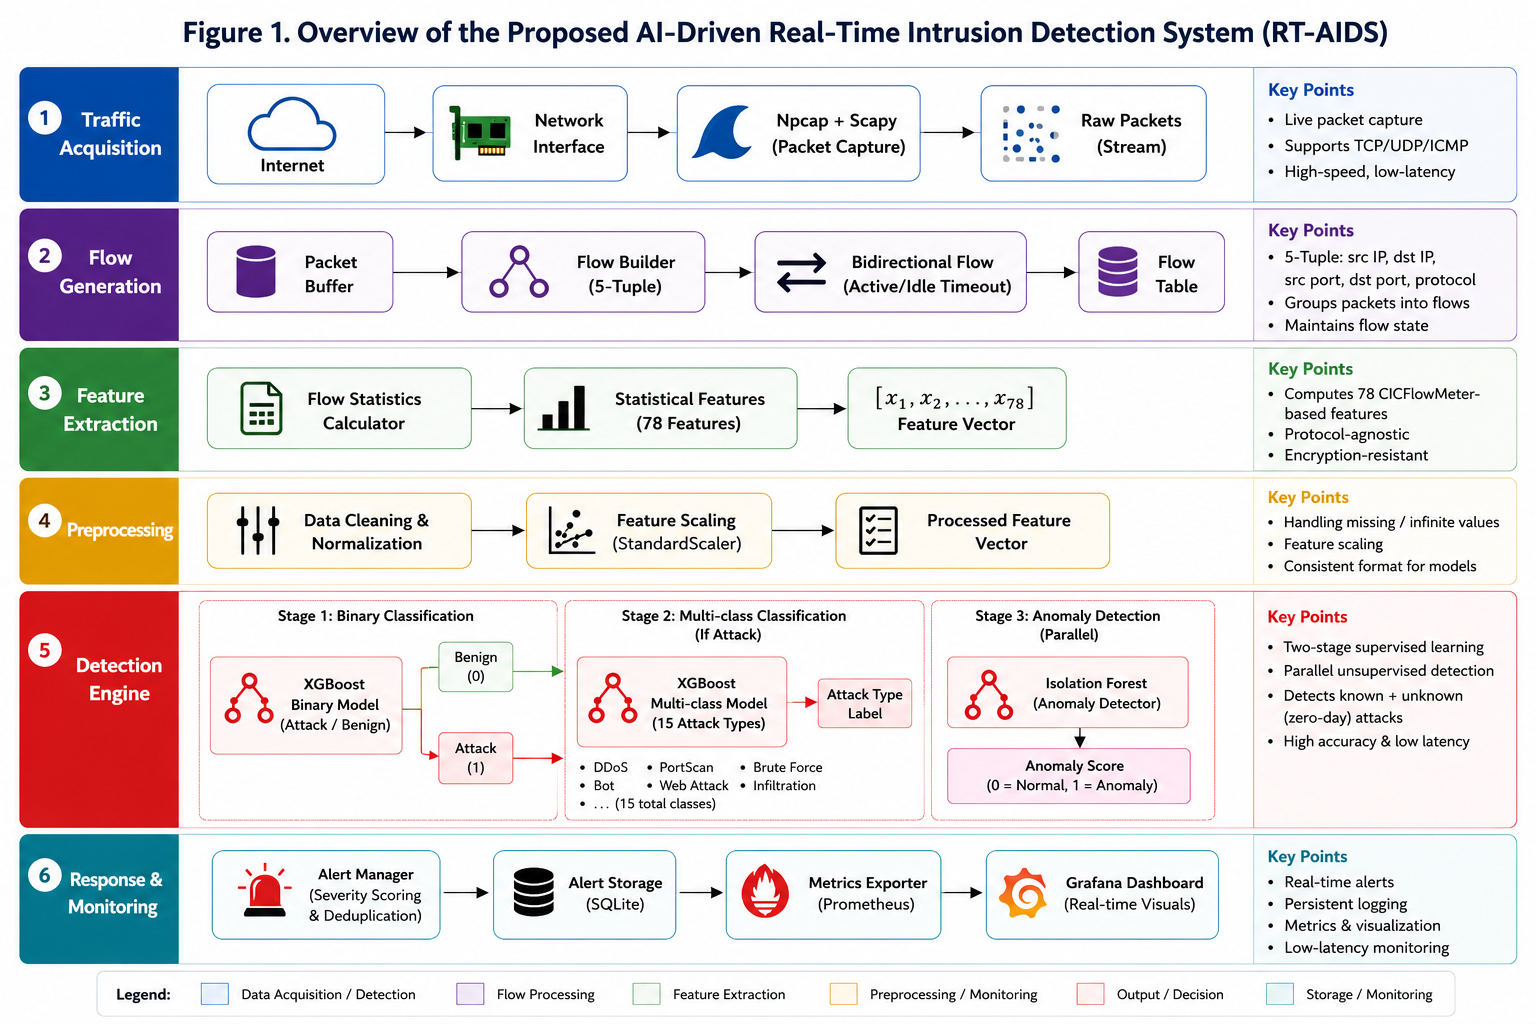
\includegraphics[width=\textwidth]{figures/figure1.Overview.png}
\caption{Overall Architecture of the Proposed AI-RTIDS System.}
\label{fig:core_pipeline}
\end{figure}

% -----------------------------------------------------------------------------
\subsection{Figure 2: ML Training Pipeline}
% -----------------------------------------------------------------------------
Figure~\ref{fig:training_pipeline} shows the seven sequential training phases, from raw dataset ingestion through preprocessing, model training, evaluation, and artifact export.
\begin{figure}[H]
\centering
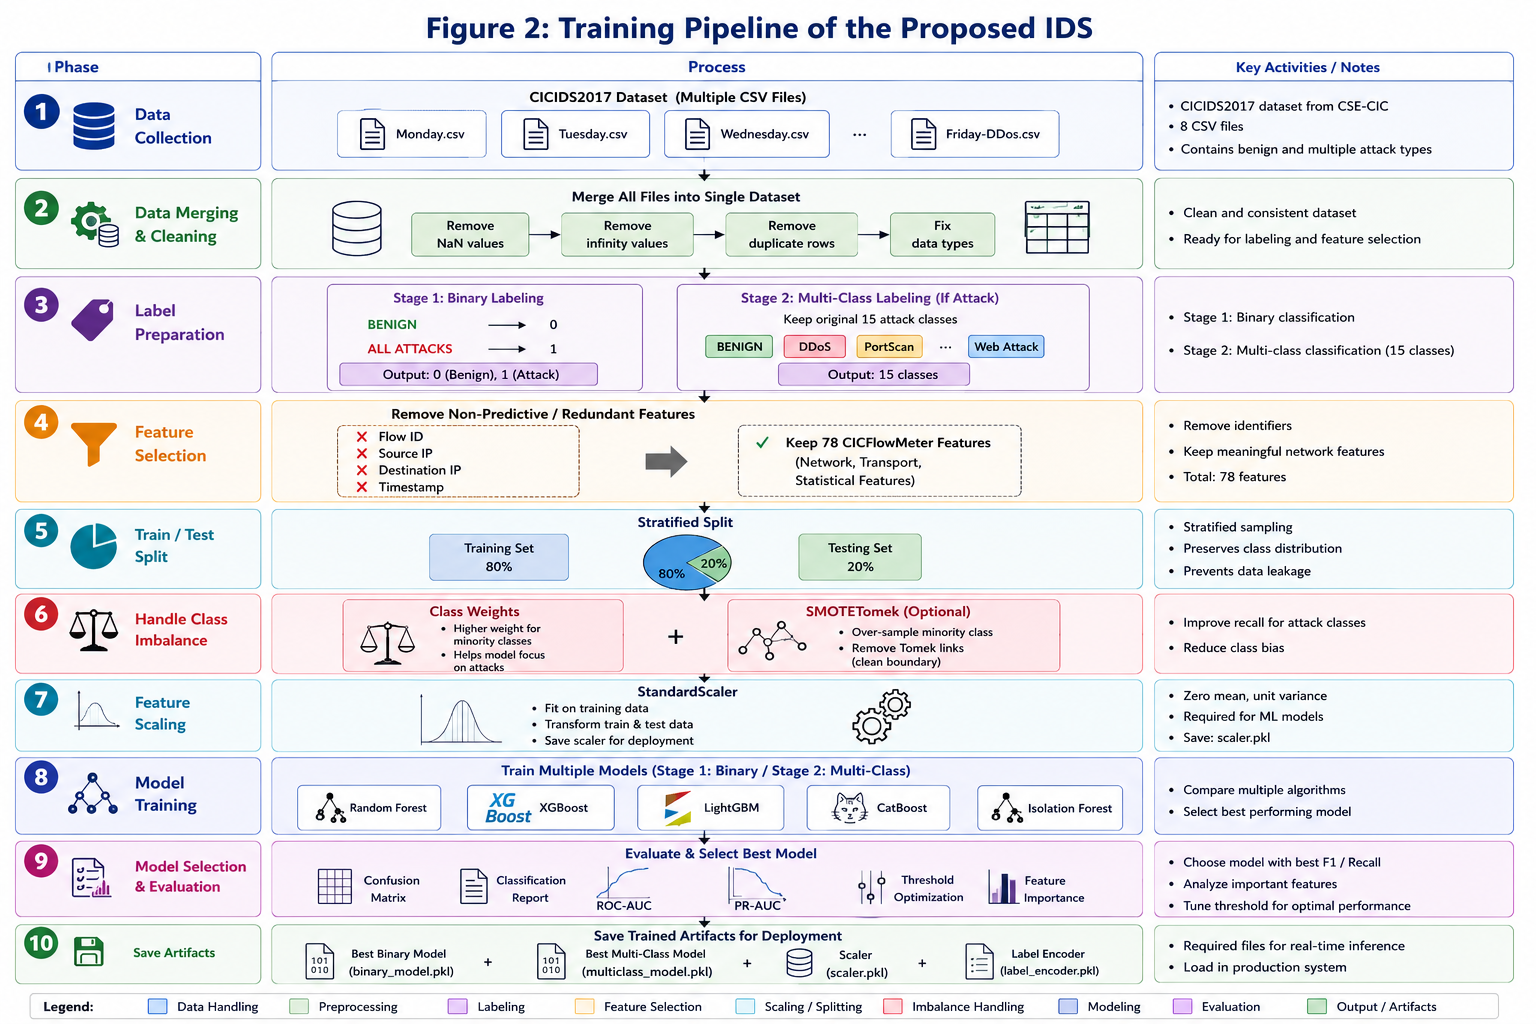
\includegraphics[width=0.85\textwidth]{figures/figure2.training_pipeline.png}
\caption{Machine Learning Training Pipeline (Seven Sequential Phases).}
\label{fig:training_pipeline}
\end{figure}

% -----------------------------------------------------------------------------
\subsection{Figure 3: Real-Time Detection Pipeline}
% -----------------------------------------------------------------------------
Figure~\ref{fig:realtime_pipeline} depicts the end-to-end runtime pipeline from live packet capture through flow aggregation, feature extraction, dual-stage inference, and alert generation.
\begin{figure}[H]
\centering
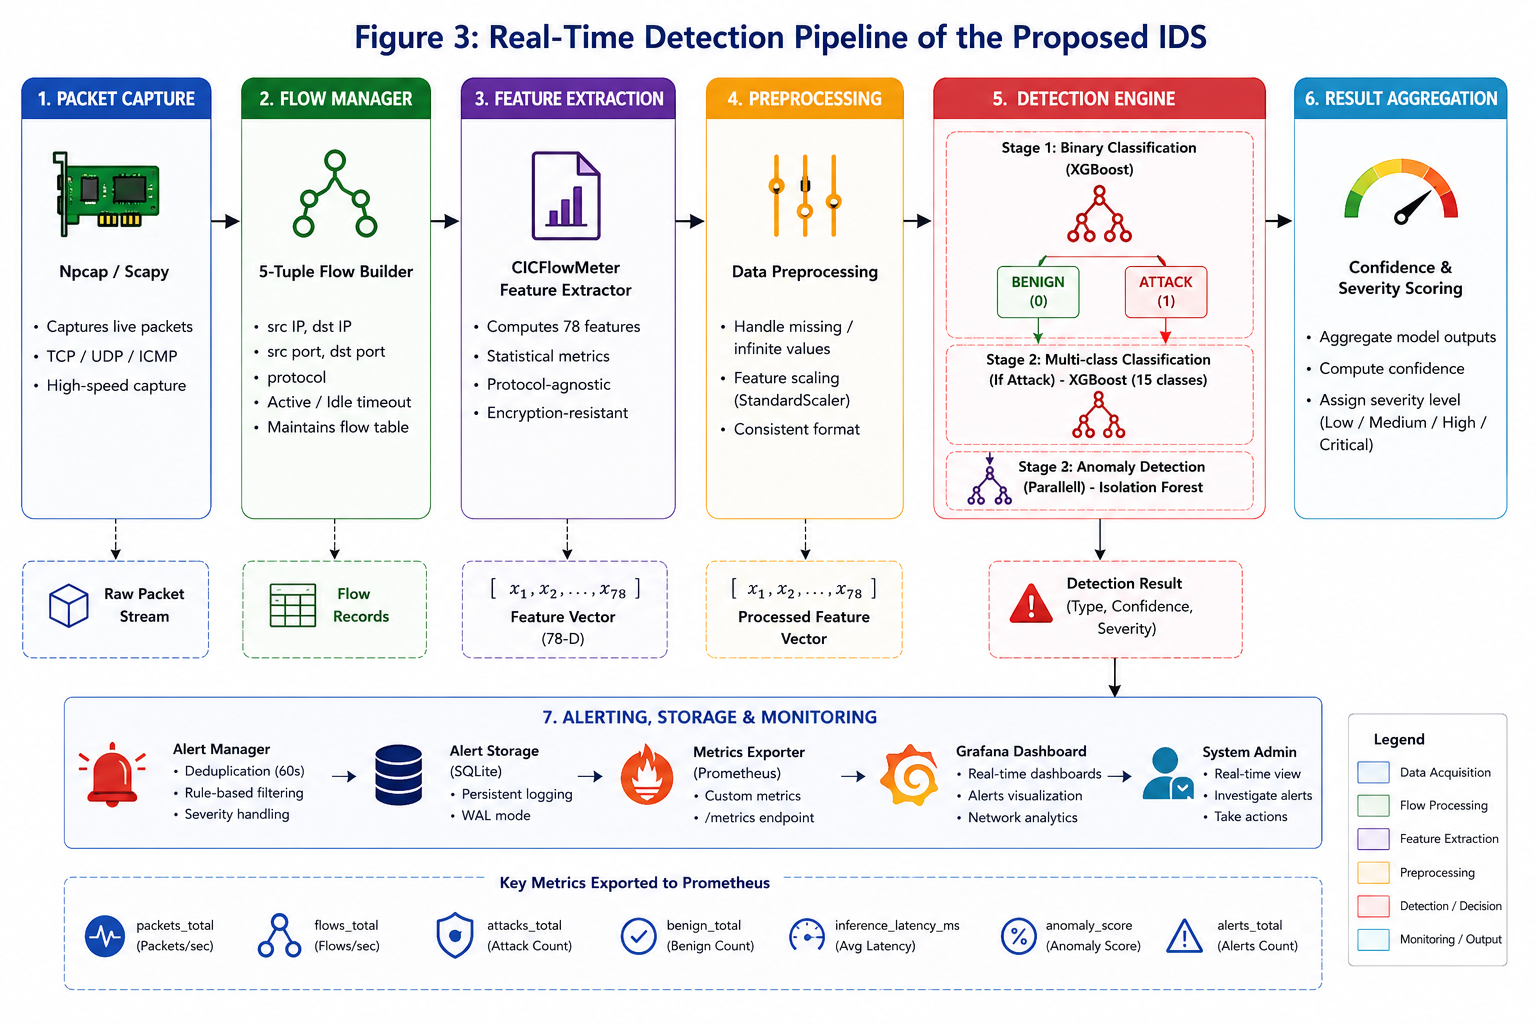
\includegraphics[width=\textwidth]{figures/figure3.real_time_detection_pipeline_of_proposed_ids.png}
\caption{Real-Time Detection Pipeline from Packet Capture to Alerting.}
\label{fig:realtime_pipeline}
\end{figure}

% -----------------------------------------------------------------------------
\subsection{Figure 4: Binary Classification Flow}
% -----------------------------------------------------------------------------
Figure~\ref{fig:binary_flow} illustrates the binary XGBoost screening stage, highlighting the early-exit path for BENIGN flows that avoids the more expensive multiclass inference.
\begin{figure}[H]
\centering
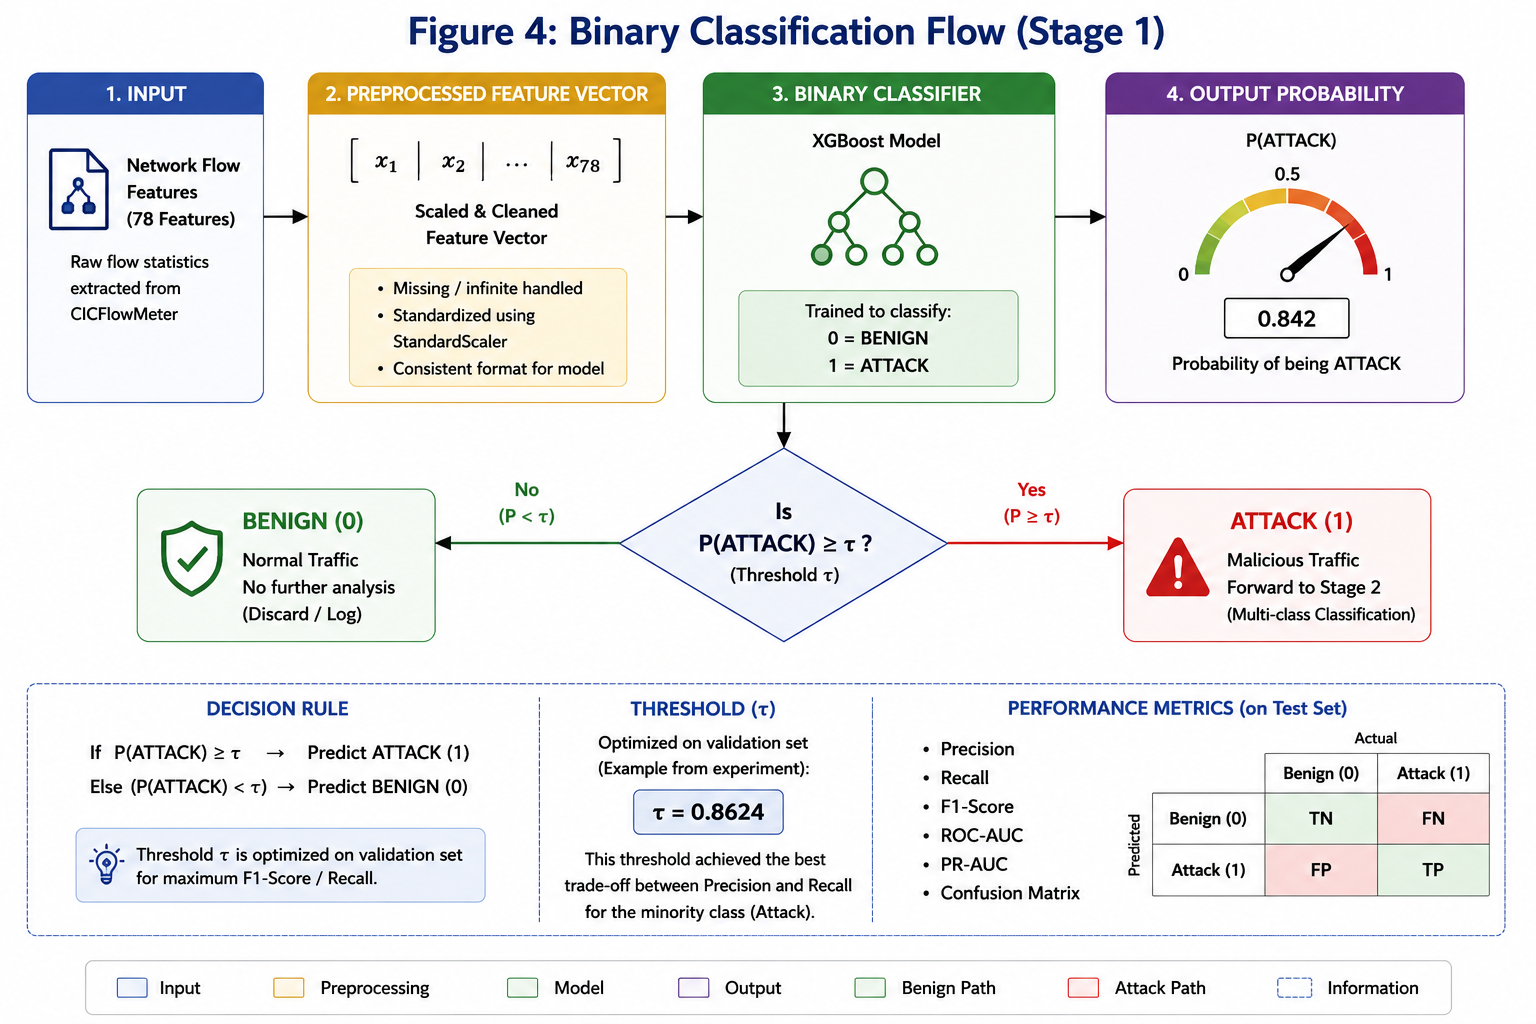
\includegraphics[width=0.85\textwidth]{figures/figure4.binary_classification_flow.png}
\caption{Binary Classification Flow with Threshold-Based Early Exit.}
\label{fig:binary_flow}
\end{figure}

% -----------------------------------------------------------------------------
\subsection{Figure 5: Multiclass Classification Flow}
% -----------------------------------------------------------------------------
Figure~\ref{fig:multiclass_flow} shows the ATTACK branch, where the 15-class XGBoost model identifies the attack type and the Isolation Forest contributes an anomaly score for composite severity calculation.
\begin{figure}[H]
\centering
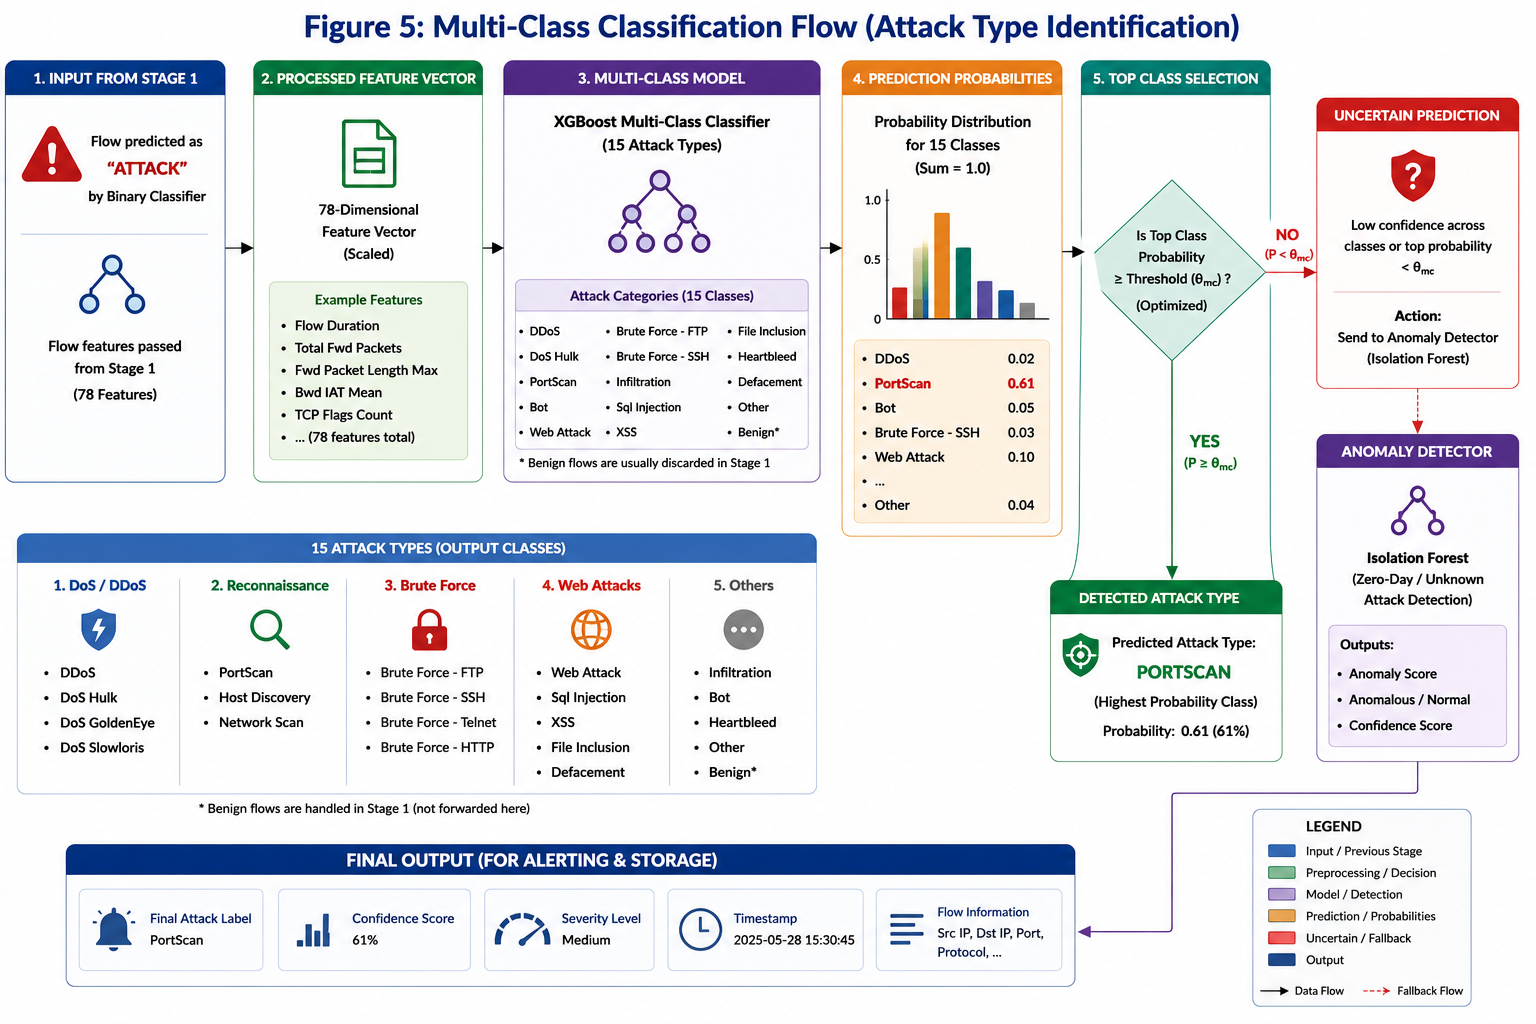
\includegraphics[width=0.85\textwidth]{figures/figure5.multi_class_classification_flow.png}
\caption{Multiclass Classification and Anomaly Detection Flow.}
\label{fig:multiclass_flow}
\end{figure}

% -----------------------------------------------------------------------------
\subsection{Figure 6: Feature Extraction Process}
% -----------------------------------------------------------------------------
Figure~\ref{fig:feature_extraction} details how 78 CICFlowMeter-compatible statistical features are computed from a completed bidirectional network flow.
\begin{figure}[H]
\centering
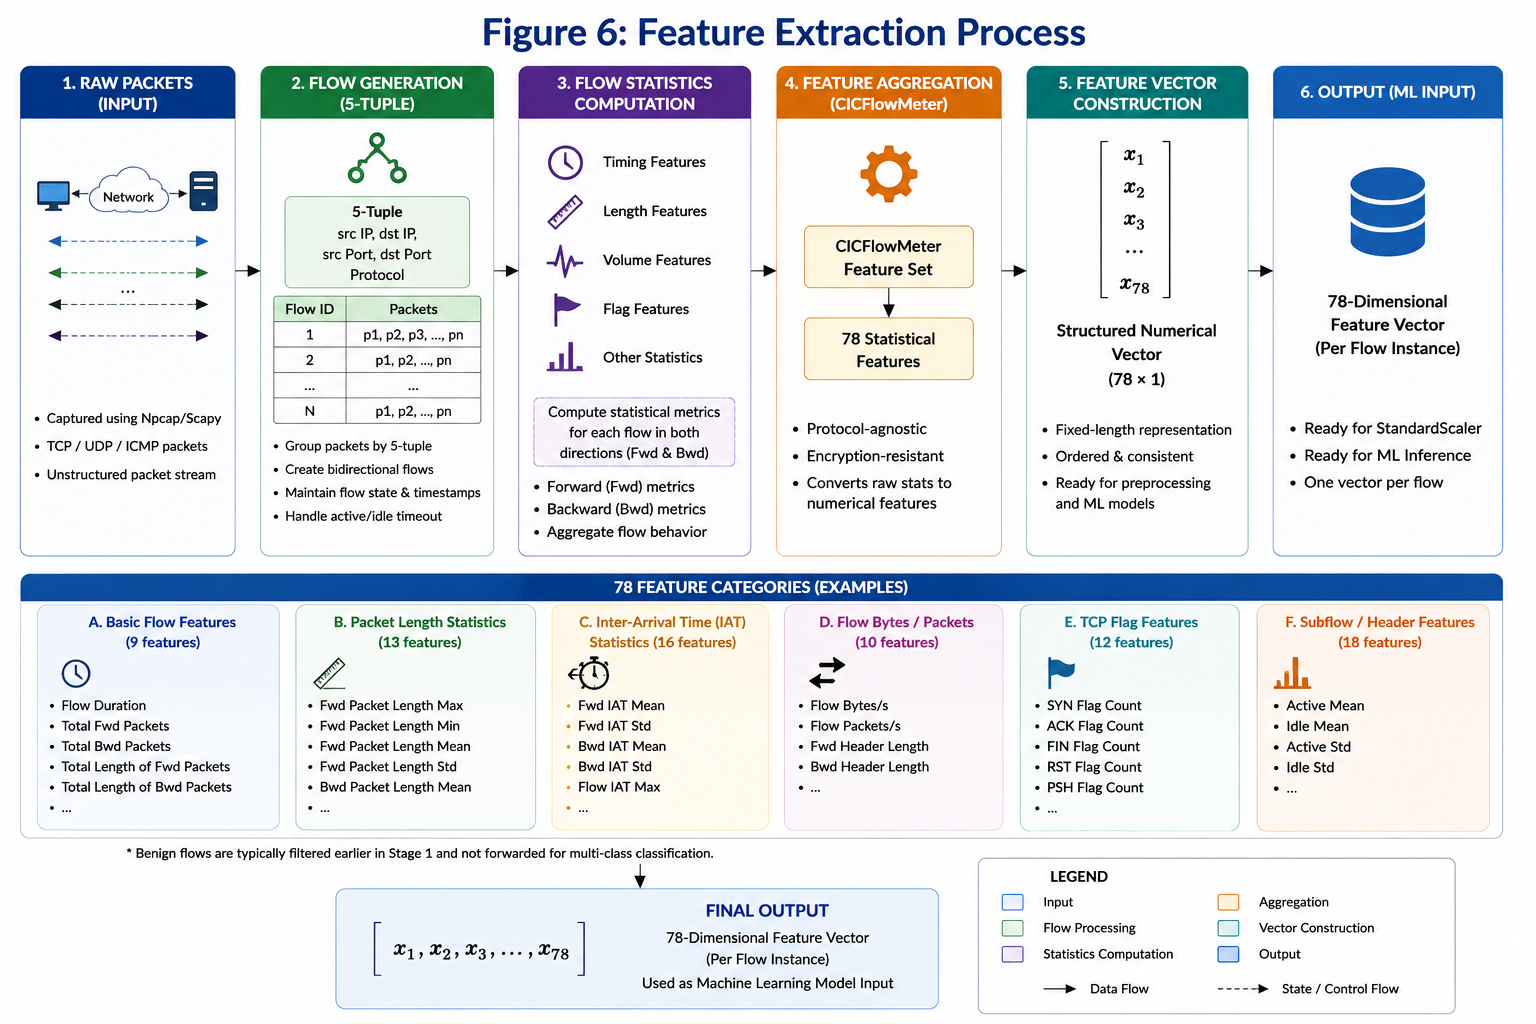
\includegraphics[width=0.85\textwidth]{figures/figure6.feature_extraction_process.png}
\caption{Feature Extraction Process (78 CICFlowMeter Features).}
\label{fig:feature_extraction}
\end{figure}

% -----------------------------------------------------------------------------
\subsection{Figure 7: Monitoring Architecture}
% -----------------------------------------------------------------------------
Figure~\ref{fig:monitoring_arch} shows how the Prometheus metrics exporter feeds the Grafana visualization stack, enabling real-time observability of detection throughput, alert rates, and system resources.
\begin{figure}[H]
\centering
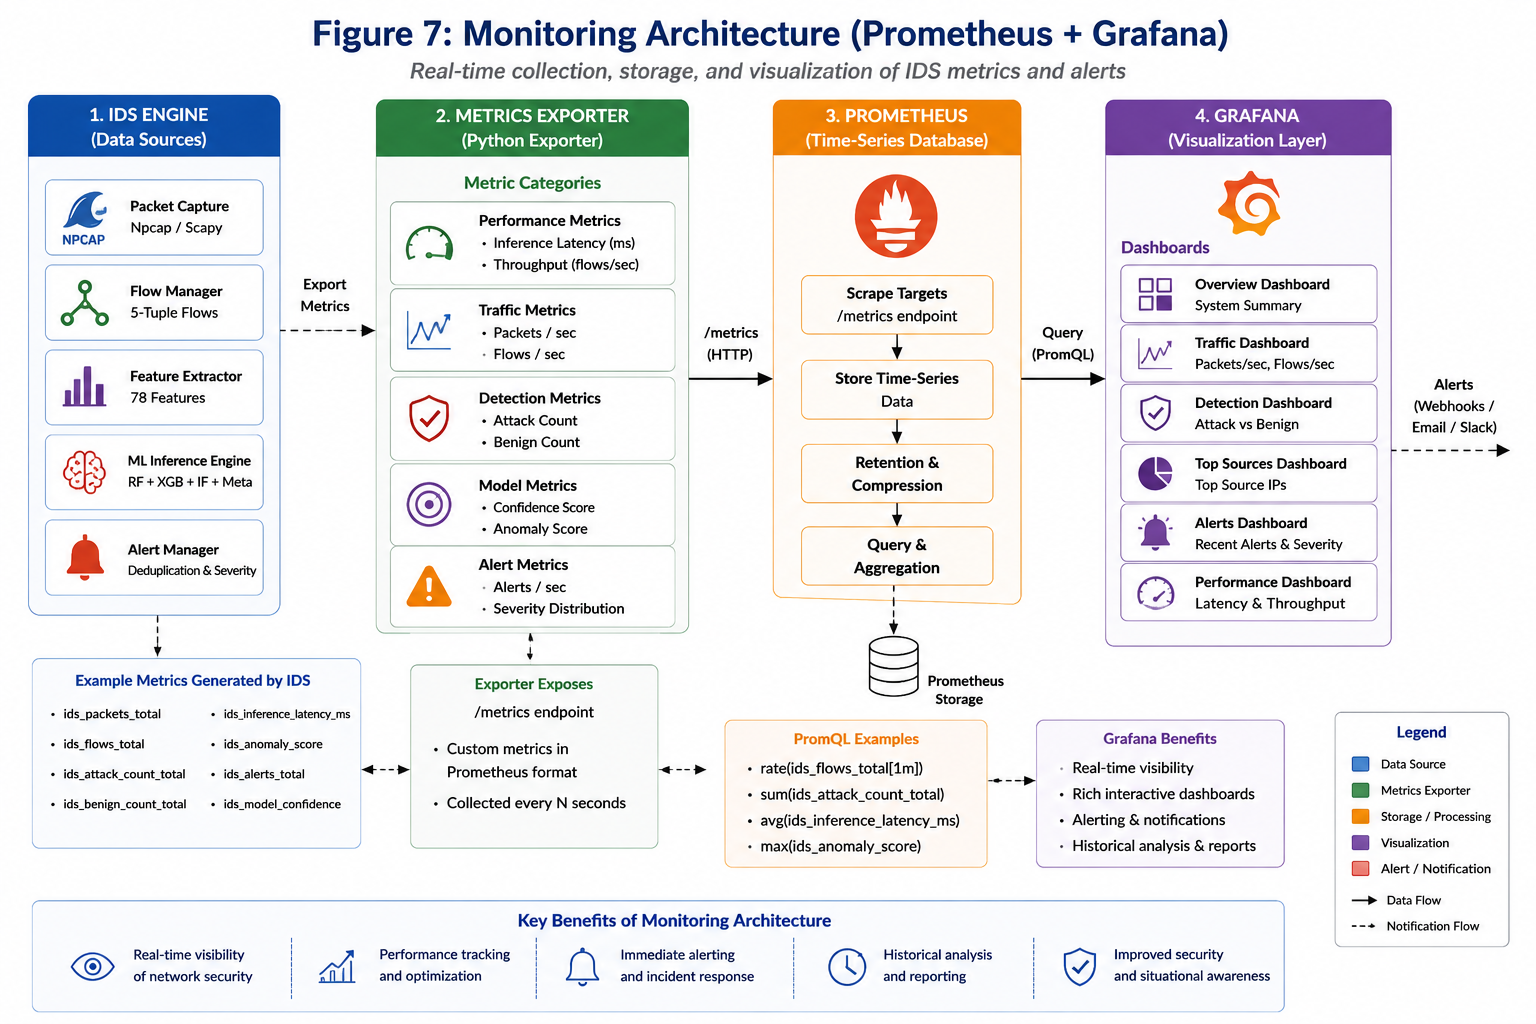
\includegraphics[width=0.85\textwidth]{figures/figure7.monitoring_architecture.png}
\caption{Monitoring Architecture with Prometheus and Grafana.}
\label{fig:monitoring_arch}
\end{figure}

% -----------------------------------------------------------------------------
\subsection{Figure 8: Complete Deployment Architecture}
% -----------------------------------------------------------------------------
Figure~\ref{fig:full_architecture} presents the complete deployment view, integrating all core and supporting components within a Docker Compose environment.
\begin{figure}[H]
\centering
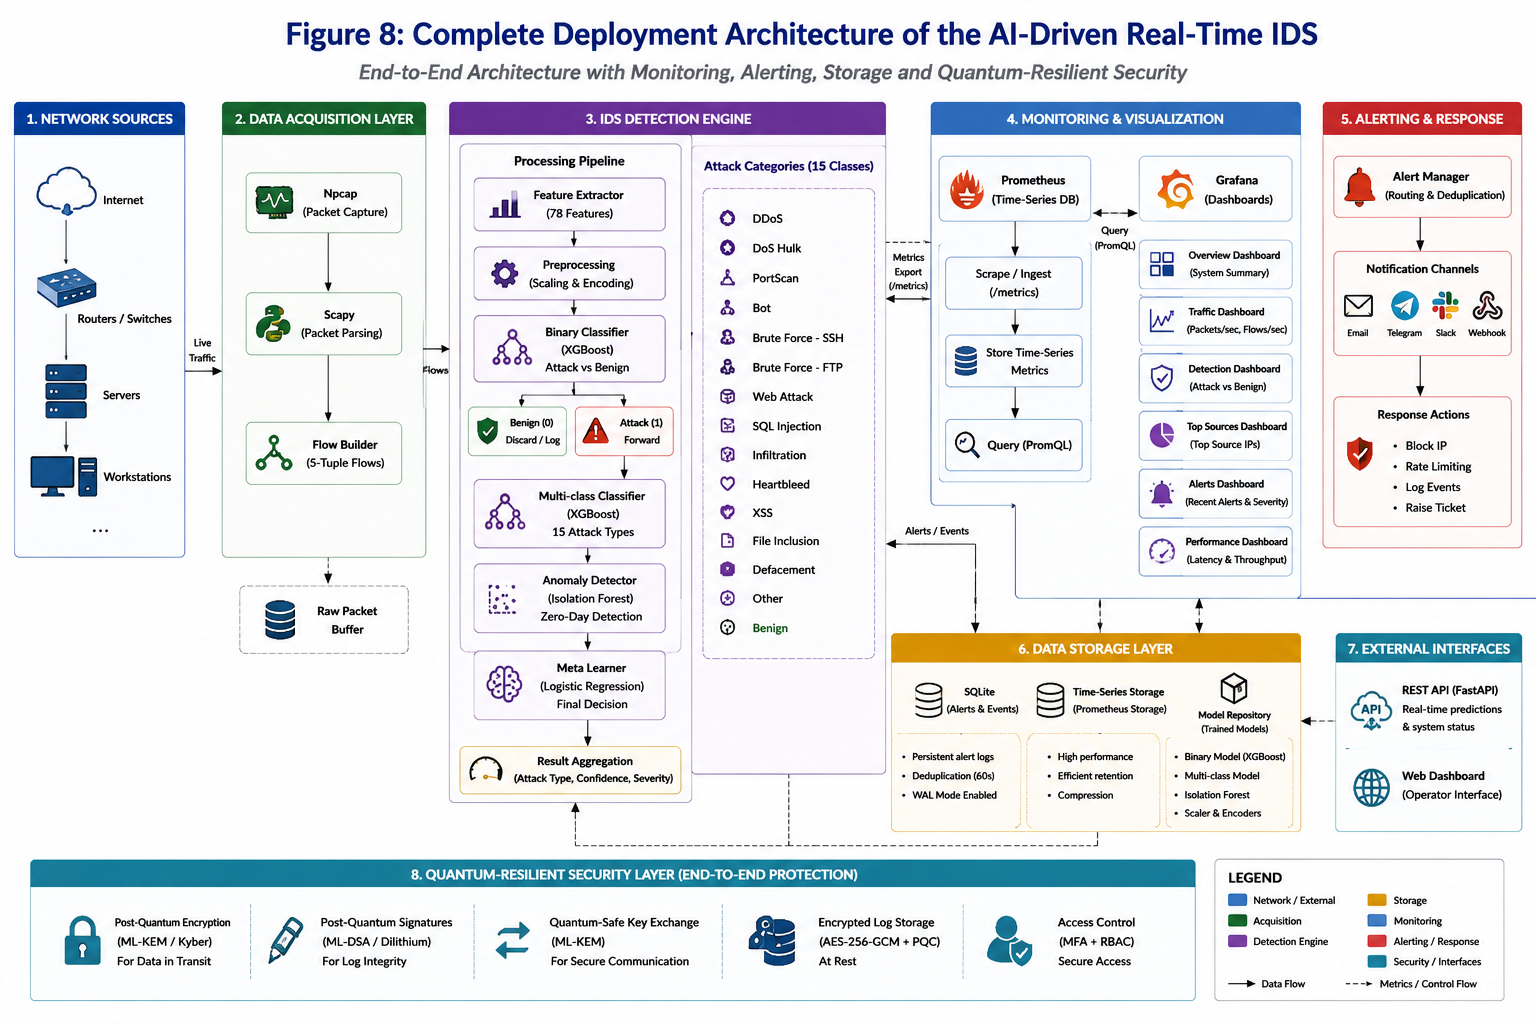
\includegraphics[width=\textwidth]{figures/figure8.complete_deployment_architecture_ai_real_time_ids.png}
\caption{Complete Deployment Architecture of the AI-RTIDS System.}
\label{fig:full_architecture}
\end{figure}

% ============================================================================
% SECTION 4: DATASET AND PREPROCESSING
% ============================================================================
\section{Dataset and Preprocessing}

\subsection{Dataset Overview: CIC-IDS-2017}

The CIC-IDS-2017 dataset, developed by the Canadian Institute for Cybersecurity, provides comprehensive network attack representation \cite{sharafaldin2018toward}:

\begin{table}[H]
\centering
\caption{CIC-IDS-2017 Dataset Properties}
\label{tab:dataset_properties}
\begin{tabular}{|l|r|}
\hline
\textbf{Property} & \textbf{Value} \\
\hline
Total Samples & 2,830,743 \\
Features & 78 (CICFlowMeter) \\
Attack Classes & 15 \\
Benign/Attack Ratio & 5.04:1 \\
Time Span & 5 days \\
Network Topology & Enterprise network \\
\hline
\end{tabular}
\end{table}

\subsection{Attack Class Distribution}

\begin{table}[H]
\centering
\caption{Attack Class Distribution}
\label{tab:attack_distribution}
\begin{tabular}{|l|r|r|}
\hline
\textbf{Class} & \textbf{Samples} & \textbf{Percentage} \\
\hline
BENIGN & 2,273,097 & 80.30\% \\
DoS Hulk & 231,399 & 8.17\% \\
PortScan & 158,930 & 5.61\% \\
DDoS & 128,027 & 4.52\% \\
DoS GoldenEye & 10,293 & 0.36\% \\
FTP-Patator & 7,938 & 0.28\% \\
SSH-Patator & 5,897 & 0.21\% \\
DoS slowloris & 5,796 & 0.20\% \\
DoS Slowhttptest & 5,499 & 0.19\% \\
Bot & 2,046 & 0.07\% \\
Web Attack - Brute Force & 1,507 & 0.05\% \\
Web Attack - XSS & 652 & 0.02\% \\
Infiltration & 36 & 0.001\% \\
Web Attack - Sql Injection & 21 & 0.001\% \\
Heartbleed & 11 & 0.0004\% \\
\hline
\end{tabular}
\end{table}

\subsection{Data Preprocessing Pipeline}

\subsubsection{Data Cleaning}

The following data cleaning steps were performed:

\begin{enumerate}
    \item Read CSV files with optimized dtypes (float32 for numeric)
    \item Strip column names of whitespace
    \item Replace "Infinity" and "-Infinity" with NaN
    \item Impute missing values with column medians
    \item Remove duplicate rows
    \item Clean label column (strip whitespace, replace special characters)
    \item Downcast numeric columns to float32/int32
\end{enumerate}

\subsubsection{Feature Management}

All 78 CICFlowMeter-compatible features are retained for the real-time inference pipeline. Median imputation is used for handling missing values during inference, ensuring robustness in live deployment scenarios.

\subsection{Dataset Limitations}

While CIC-IDS-2017 is one of the most comprehensive public datasets, it has several limitations that affect generalization:
\begin{itemize}
    \item \textbf{Enterprise-only traffic}: The dataset represents a single enterprise network topology; performance on other network architectures (e.g., data centers, IoT) may vary.
    \item \textbf{Timeliness}: The data was captured in 2017; modern attack techniques and network protocols may not be fully represented.
    \item \textbf{Encrypted traffic}: The dataset contains limited encrypted traffic analysis, which may reduce detection capability for encrypted attacks.
    \item \textbf{Rare classes}: Extremely rare attack types (e.g., Heartbleed with only 11 samples) are insufficient for robust model learning.
\end{itemize}
These limitations are acknowledged and should be considered when interpreting the results.

\subsection{Dataset Split Strategy}

For binary classification, a stratified 80/20 split is applied:
\begin{itemize}
    \item Train: 80\% (2,259,069 samples)
    \item Test: 20\% (514,812 samples)
\end{itemize}

For multiclass classification, a stratified 70/10/20 split is applied:
\begin{itemize}
    \item Train: 70\% ($\approx$1,981,520 samples)
    \item Validation: 10\% ($\approx$283,074 samples)
    \item Test: 20\% (514,812 samples)
\end{itemize}

All splits use \texttt{stratify=y} to preserve class proportions. Test sets are saved before training begins, ensuring strict evaluation integrity.

% ============================================================================
% SECTION 5: MACHINE LEARNING MODELS
% ============================================================================
\section{Machine Learning Models}

\subsection{Model Selection}

\begin{table}[H]
\centering
\caption{Model Selection Criteria}
\label{tab:model_selection}
\begin{tabular}{|p{3cm}|p{4cm}|p{4cm}|}
\hline
\textbf{Criterion} & \textbf{Requirement} & \textbf{Selected Model} \\
\hline
High Accuracy & $>$99\% & XGBoost \\
Interpretability & Feature importance & XGBoost, Random Forest \\
Anomaly Detection & Zero-day detection & Isolation Forest \\
Resource Efficiency & Low memory footprint & XGBoost \\
\hline
\end{tabular}
\end{table}

\subsection{XGBoost Binary Classifier}

\begin{lstlisting}[language=Python, caption=XGBoost Binary Classifier Configuration]
xgb_binary = XGBClassifier(
    n_estimators=300,
    max_depth=8,
    learning_rate=0.05,
    subsample=0.8,
    colsample_bytree=0.8,
    scale_pos_weight=5.04,  # BENIGN:ATTACK ratio
    reg_alpha=0.5,
    reg_lambda=1.0,
    eval_metric="logloss",
    tree_method="hist",
    random_state=42
)
\end{lstlisting}

\subsection{XGBoost Multiclass Classifier}

\begin{lstlisting}[language=Python, caption=XGBoost Multiclass Classifier Configuration]
xgb_multiclass = XGBClassifier(
    objective="multi:softprob",
    num_class=15,
    n_estimators=300,
    max_depth=6,
    learning_rate=0.05,
    subsample=0.8,
    colsample_bytree=0.8,
    reg_alpha=0.5,
    reg_lambda=1.0,
    eval_metric="mlogloss",
    tree_method="hist",
    random_state=42
)
\end{lstlisting}

\subsection{Isolation Forest Anomaly Detector}

\begin{lstlisting}[language=Python, caption=Isolation Forest Configuration]
iso_model = IsolationForest(
    n_estimators=200,
    contamination="auto",
    random_state=42
)
\end{lstlisting}

\subsection{Model Comparison}

\begin{table}[H]
\centering
\caption{Model Performance Comparison (on held-out test set)}
\label{tab:model_comparison}
\begin{tabular}{|l|r|r|r|}
\hline
\textbf{Model} & \textbf{Accuracy} & \textbf{F1-Score} & \textbf{Model Size} \\
\hline
XGBoost Binary & 99.84\% & 99.74\% & 1.47 MB \\
Random Forest Binary & 99.40\% & 99.65\% & 76.10 MB \\
Isolation Forest & N/A & 58.19\% & 1.42 MB \\
XGBoost Multiclass & 99.84\% & 99.85\% (w) & 8.69 MB \\
\hline
\end{tabular}
\end{table}

Based on this comparison, XGBoost was selected for the production pipeline due to its high accuracy, small model size, and fast inference. Although Random Forest is not used during deployment, it serves as a baseline model for comparative evaluation.

\subsection{Performance Metrics}

For evaluation, we employ multiple metrics because the dataset is highly imbalanced. Accuracy alone would be misleading; therefore we report Precision, Recall, F1-Score, ROC-AUC, and PR-AUC, which are standard for imbalanced classification tasks. The definitions are as follows:

\begin{equation}
\text{Accuracy} = \frac{TP + TN}{TP + TN + FP + FN}
\end{equation}
\begin{equation}
\text{Precision} = \frac{TP}{TP + FP}
\end{equation}
\begin{equation}
\text{Recall} = \frac{TP}{TP + FN}
\end{equation}
\begin{equation}
\text{F1-Score} = 2 \times \frac{\text{Precision} \times \text{Recall}}{\text{Precision} + \text{Recall}}
\end{equation}

% ============================================================================
% SECTION 6: SYSTEM IMPLEMENTATION
% ============================================================================
\section{System Implementation}

The system is implemented in Python 3.10 and follows the two-tier architecture described in Section~\ref{sec:architecture_overview}. The core detection pipeline (Packet Capture, Flow Manager, Feature Extraction, Inference, Alert Manager) is entirely self-contained. The supporting runtime infrastructure (Prometheus, FastAPI, Grafana, Worker Pool) enhances observability, scalability, and external integration, but does not affect detection logic.

% -----------------------------------------------------------------------
\subsection{Core IDS Components}
% -----------------------------------------------------------------------

\subsubsection{Packet Capture}
\label{sec:core_capture}

The packet capture module uses Scapy to capture live network packets with BPF filter support, handling TCP, UDP, and ICMP. A background flush thread expires timed-out flows every 10 seconds.

\begin{lstlisting}[language=Python, caption=Packet Capture Core Implementation]
class PacketCapture:
    def __init__(self, interface: str, on_flow_complete: Callable,
                 filter_bpf: str = "ip", idle_timeout: float = 120.0,
                 absolute_timeout: float = 600.0) -> None:
        self._flow_manager = FlowManager(on_flow_complete, idle_timeout, absolute_timeout)

    def start(self, packet_count: int = 0) -> None:
        self._running = True
        self._start_flush_thread()  # daemon: flush every 10s
        sniff(iface=self._interface, filter=self._filter, prn=self._handle_packet,
              count=packet_count, store=False, stop_filter=lambda _: not self._running)
\end{lstlisting}

\subsubsection{Flow Manager}
\label{sec:core_flow}

The Flow Manager maintains a thread-safe table of bidirectional flows using \texttt{threading.Lock}. It performs bidirectional lookup and exports flows on TCP FIN/RST, idle timeout (120s), or absolute timeout (600s).

\begin{lstlisting}[language=Python, caption=Flow Manager Bidirectional Logic]
def process_packet(self, pkt: PacketRecord, key: FlowKey) -> None:
    with self._lock:
        flow = self._flows.get(key)
        if flow is None:
            # Check reverse direction
            reverse_key = FlowKey(src_ip=key.dst_ip, dst_ip=key.src_ip,
                                  src_port=key.dst_port, dst_port=key.src_port,
                                  protocol=key.protocol)
            flow = self._flows.get(reverse_key)
            if flow:
                self._flows[key] = flow
                flow.add_packet(pkt)
                return
            flow = NetworkFlow(key=key)
            self._flows[key] = flow
        flow.add_packet(pkt)
        if pkt.tcp_flags & (_TCP_FIN | _TCP_RST):
            self._export(key, flow)
\end{lstlisting}

\subsubsection{Feature Extractor}
\label{sec:core_feature}

The feature extractor computes 78 CICFlowMeter-compatible features including basic flow statistics, packet length metrics, inter-arrival times, TCP flags, and subflow features.

\begin{lstlisting}[language=Python, caption=Feature Extraction Snippet]
def extract_features(flow: NetworkFlow) -> Dict[str, float]:
    features = {}
    features["Flow Duration"] = flow.duration
    features["Total Fwd Packets"] = len(flow.fwd_packets)
    features["Total Backward Packets"] = len(flow.bwd_packets)
    # ... additional 75 features
    return features
\end{lstlisting}

\subsubsection{Preprocessing and Inference Engine}
\label{sec:core_inference}

Preprocessing and inference are performed atomically. The \texttt{ModelManager} singleton loads all artifacts (XGBoost models, Isolation Forest, scaler, medians, encoder, thresholds) at startup from the structured \texttt{models/} directory.

\begin{table}[H]
\centering
\caption{Model Artifacts Organization and Descriptions}
\label{tab:model_artifacts}
\begin{tabular}{|l|l|p{7cm}|}
\hline
\textbf{Subdirectory} & \textbf{Artifact Name} & \textbf{Function \& Role in Runtime Pipeline} \\
\hline
\texttt{anomaly/} & \texttt{isolation\_forest.pkl} & Unsupervised Isolation Forest model for zero-day anomaly scoring ($s_{\text{iso}}$). \\
\hline
\texttt{binary/} & \texttt{xgb\_binary.pkl} & Primary XGBoost binary classifier for high-speed BENIGN vs. ATTACK screening. \\
 & \texttt{rf_binary.pkl} & Secondary Random Forest binary classifier (ensemble/evaluation). \\
 & \texttt{binary\_threshold.json} & F1-optimal probability decision thresholds (e.g., 0.8624). \\
\hline
\texttt{multiclass/} & \texttt{xgb\_multiclass.pkl} & 15-class XGBoost multiclass model for attack category identification. \\
 & \texttt{label\_encoder.pkl} & Scikit-learn LabelEncoder mapping numeric predictions to attack strings. \\
\hline
\texttt{preprocessing/} & \texttt{feature\_medians.pkl} & Median values per feature for missing value (\texttt{NaN}/\texttt{Inf}) imputation. \\
 & \texttt{multiclass\_feature\_columns.pkl} & Enforces exact 78-feature column ordering during inference. \\
 & \texttt{scaler.pkl} & Fitted StandardScaler for feature vector standardization. \\
\hline
\end{tabular}
\end{table}

\begin{lstlisting}[language=Python, caption=Inference Pipeline (predict_flow)]
def predict_flow(features: dict) -> dict:
    start = time.perf_counter()
    X_arr = np.zeros((1, len(MODELS.feature_columns)), dtype=np.float32)
    for i, col in enumerate(MODELS.feature_columns):
        val = features.get(col, 0.0)
        if math.isinf(val) or math.isnan(val):
            val = MODELS.feature_medians.get(col, 0.0)
        X_arr[0, i] = val

    attack_prob = float(MODELS.xgb_binary.predict_proba(X_arr)[0, 1])
    if attack_prob < MODELS.binary_threshold:
        return {"is_attack": False, "attack_type": "BENIGN", ...}

    # Multiclass classification
    multi_probs = MODELS.xgb_multiclass.predict_proba(X_arr)[0]
    class_idx = int(np.argmax(multi_probs))
    attack_type = str(MODELS.label_encoder.inverse_transform([class_idx])[0])
    attack_confidence = float(np.max(multi_probs))

    # Isolation Forest anomaly score (computed after multiclass)
    iso_score = compute_iso_score(X_arr)
    severity = calculate_severity(attack_prob, iso_score)
    return {"is_attack": True, "attack_type": attack_type,
            "attack_confidence": attack_confidence,
            "iso_score": iso_score, "severity": severity, ...}
\end{lstlisting}

\subsubsection{Alert Manager}
\label{sec:core_alert}

The Alert Manager orchestrates rule filtering, 60-second deduplication (keyed by \texttt{src\_ip}, \texttt{dst\_ip}, \texttt{attack\_type}), severity scoring, SQLite persistence (WAL mode), optional real-time Telegram Bot notifications, and WebSocket streaming.

\begin{lstlisting}[language=Python, caption=Alert Manager Process Logic]
def process(self, prediction: dict, flow: NetworkFlow) -> Optional[Alert]:
    if not self._rules.should_alert(prediction, dst_port=flow.key.dst_port):
        return None
    dedup_key = (flow.key.src_ip, flow.key.dst_ip, prediction["attack_type"])
    with self._lock:
        if self._dedup_cache.get(dedup_key) and (time.time() - ...) < 60:
            return None
        self._dedup_cache[dedup_key] = time.time()
    alert = Alert(...)
    self._storage.insert(alert)
    return alert
\end{lstlisting}

% -----------------------------------------------------------------------
\subsection{Supporting Runtime Infrastructure}
% -----------------------------------------------------------------------

\subsubsection{Prometheus Metrics}
\label{sec:sup_metrics}

The monitoring subsystem exports 15 metrics including packet/flow counters, prediction latency histograms, attack type counters, and system resource gauges.

\begin{lstlisting}[language=Python, caption=Prometheus Metrics Definitions]
# Counters (9)
packets_processed = Counter("ids_packets_processed_total", "...")
flows_completed = Counter("ids_flows_completed_total", "...")
predictions_total = Counter("ids_predictions_total", "...")
attacks_detected = Counter("ids_attacks_detected_total", "...")
benign_detected = Counter("ids_benign_detected_total", "...")
alerts_total = Counter("ids_alerts_total", "...")
alerts_deduped = Counter("ids_alerts_deduped_total", "...")
attack_type_total = Counter("ids_attack_type_total", "...", ["type"])
alerts_severity_total = Counter("ids_alerts_severity_total", "...", ["severity"])

# Histograms (2)
inference_latency = Histogram("ids_inference_latency_ms", "...",
                              buckets=[0.1, 0.5, 1, 2, 5, 10, 20, 50, 100, 200, 500])
feature_latency = Histogram("ids_feature_extraction_latency_ms", "...")

# Gauges (4)
active_flows = Gauge("ids_active_flows", "...")
alert_rate = Gauge("ids_alert_rate", "...")
cpu_usage = Gauge("ids_cpu_usage_percent", "...")
memory_usage = Gauge("ids_memory_usage_percent", "...")
\end{lstlisting}

\subsubsection{FastAPI REST/WebSocket Interface}
\label{sec:sup_api}

The optional API layer provides six endpoints: \texttt{GET /health}, \texttt{GET /stats}, \texttt{GET /alerts}, \texttt{GET /models}, \texttt{POST /predict}, and \texttt{WS /stream} for real-time alert broadcasting.

\subsubsection{Inference Worker Pool}
\label{sec:sup_pool}

The multi-threaded worker pool (\texttt{--workers N}) provides linear scalability. Single-thread throughput is 197 pred/sec (experimentally measured). Based on measured single-thread performance, the projected aggregate throughput is approximately 2700 flows/sec at 14 workers, assuming ideal near-linear scaling. The worker count is configurable at runtime, allowing deployments to balance throughput and available hardware resources.

\subsubsection{Grafana and Docker Compose}
\label{sec:sup_grafana}

A Docker Compose stack provisions Prometheus (container port \texttt{9091:9090}) and Grafana (host port \texttt{3001:3000}) with automated provisioning. The Grafana stack integrates two primary data sources:
\begin{enumerate}
    \item \textbf{Prometheus}: Connected directly to \texttt{http://prometheus:9090} to query live flow metrics, throughput histograms, CPU/memory usage, and attack distribution counters.
    \item \textbf{SQLite}: Powered by the \texttt{frser-sqlite-datasource} plugin mapping container directory \texttt{/data/alerts/alerts.db} to visualize persistent historical alert records, severity breakdowns, and source/destination IP heatmaps.
\end{enumerate}
The pre-built \texttt{ids\_dashboard.json} dashboard provides a centralized, real-time command center for security operators.

% -----------------------------------------------------------------------
\subsection{Runtime Workflow (End-to-End)}
% -----------------------------------------------------------------------

\begin{algorithm}[H]
\caption{Runtime Packet Processing Workflow}
\label{alg:runtime}
\begin{algorithmic}[1]
\Procedure{ProcessPacket}{packet}
    \State Extract 5-tuple (\texttt{sip}, \texttt{dip}, \texttt{sport}, \texttt{dport}, \texttt{proto})
    \State Find or create flow in FlowManager
    \State Add packet to flow
    \If{flow is complete}
        \State Extract 78 features
        \State \Call{RunInference}{features} \Comment{Binary $\rightarrow$ Multi $\rightarrow$ IF}
        \State Generate alert if needed
        \State Export metrics to Prometheus
    \EndIf
\EndProcedure
\end{algorithmic}
\end{algorithm}

% -----------------------------------------------------------------------
\subsection{System Demonstration Outputs}
% -----------------------------------------------------------------------

\begin{figure}[H]
\centering
\includegraphics[width=0.92\textwidth]{terminal_output.png}
\caption{Terminal Output showing real-time classification and alerts.}
\label{fig:terminal_output}
\end{figure}

\begin{figure}[H]
\centering
\includegraphics[width=0.92\textwidth]{sqlite_output.png}
\caption{SQLite Alert Database showing persisted alert records.}
\label{fig:sqlite_output}
\end{figure}

\begin{figure}[H]
\centering
\includegraphics[width=0.92\textwidth]{prometheus_output.png}
\caption{Prometheus Metrics Endpoint showing exported IDS metrics.}
\label{fig:prometheus_output}
\end{figure}

\newpage
\section{Experimental Results and Analysis}

\subsection{Experimental Setup}

\textbf{Training Hardware}: Intel Core i7-8550U, 16 GB RAM, Windows 11. \\
\textbf{Target Deployment}: 8 GB RAM, standard CPU, Npcap/libpcap. \\
\textbf{Software}: Python 3.10, XGBoost 1.7.0, Scikit-learn 1.2.0, Pandas 1.5.0, Scapy 2.4.5, FastAPI 0.103.0.

\subsection{Binary Classification Results}

\subsubsection{XGBoost Binary}

\begin{table}[H]
\centering
\caption{XGBoost Binary Classification Performance}
\label{tab:xgb_binary_results}
\begin{tabular}{|l|r|}
\hline
\textbf{Metric} & \textbf{Value} \\
\hline
Test Records & 514,812 \\
Accuracy & 99.92\% \\
Precision & 99.68\% \\
Recall & 99.81\% \\
F1-Score & 99.74\% \\
False Positive Rate (FPR) & 0.064\% (277) \\
False Negative Rate (FNR) & 0.19\% (159) \\
ROC-AUC & 0.9999 \\
PR-AUC & 0.9999 \\
F1-Optimal Threshold & 0.8624 \\
\hline
\end{tabular}
\end{table}

\begin{figure}[H]
\centering
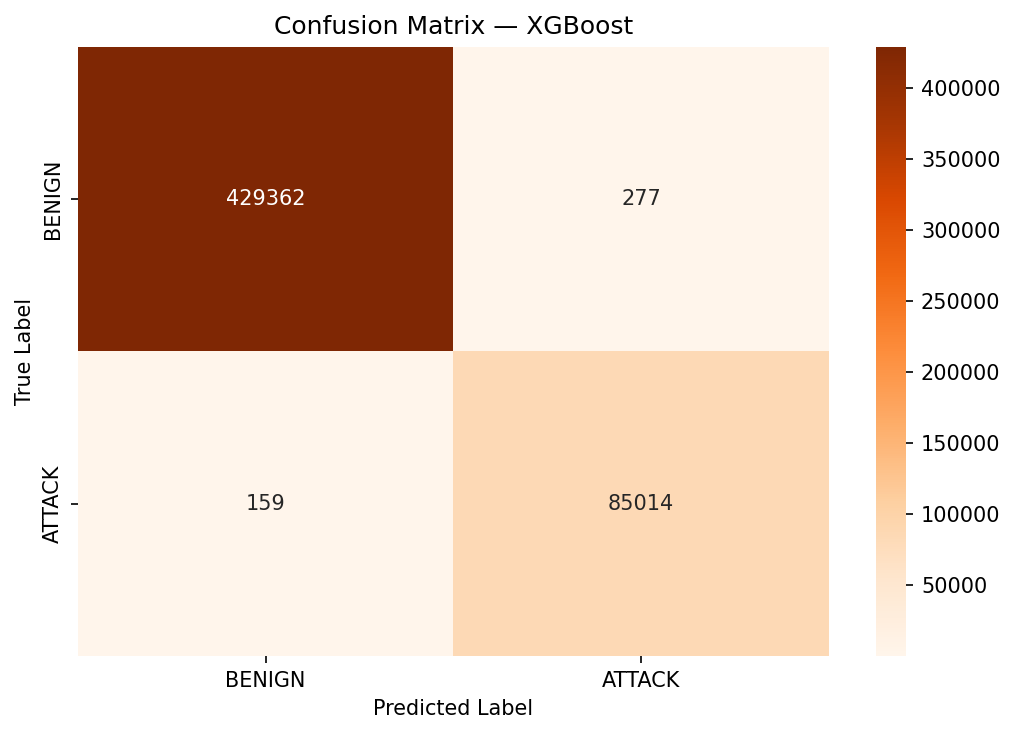
\includegraphics[width=0.80\textwidth]{results/confusion_matrix_xgb.png}
\caption{Confusion Matrix for XGBoost Binary Classifier.}
\label{fig:cm_xgb}
\end{figure}

\subsubsection{Random Forest Binary}

\begin{table}[H]
\centering
\caption{Random Forest Binary Classification Performance}
\label{tab:rf_binary_results}
\begin{tabular}{|l|r|}
\hline
\textbf{Metric} & \textbf{Value} \\
\hline
Test Records & 514,812 \\
Accuracy & 99.89\% \\
Precision & 99.53\% \\
Recall & 99.78\% \\
F1-Score & 99.66\% \\
False Positive Rate (FPR) & 0.093\% (398) \\
False Negative Rate (FNR) & 0.22\% (191) \\
ROC-AUC & 0.9999 \\
PR-AUC & 0.9998 \\
F1-Optimal Threshold & 0.5991 \\
\hline
\end{tabular}
\end{table}

\begin{figure}[H]
\centering
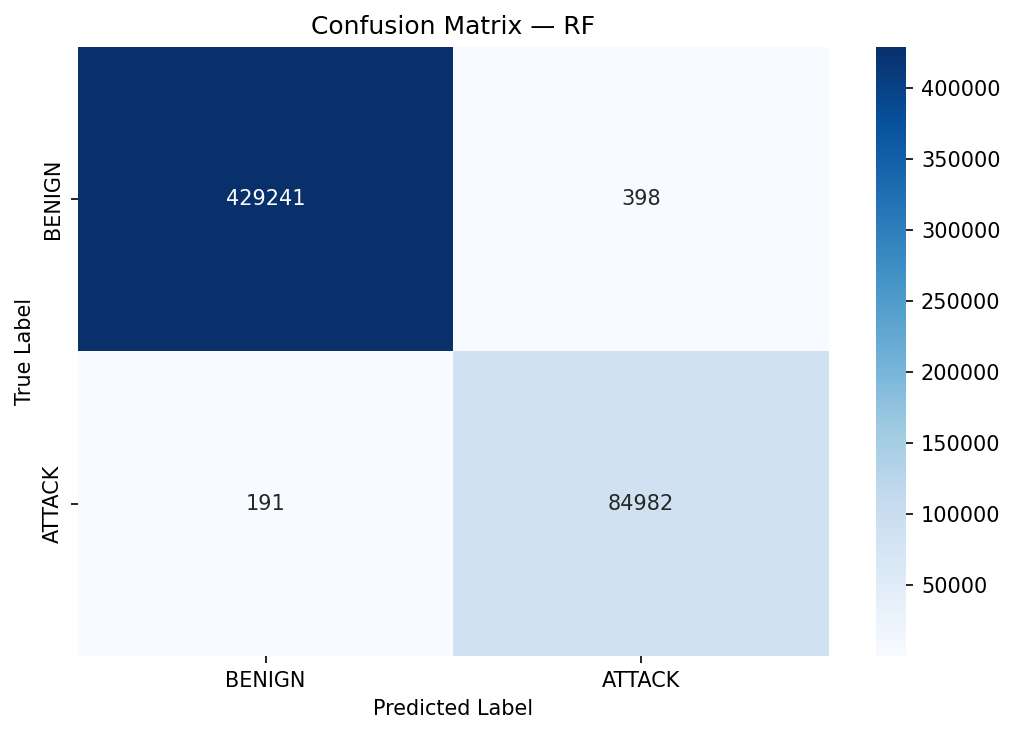
\includegraphics[width=0.80\textwidth]{results/confusion_matrix_rf.png}
\caption{Confusion Matrix for Random Forest Binary Classifier.}
\label{fig:cm_rf}
\end{figure}

\subsubsection{Isolation Forest Anomaly Detection}

\begin{table}[H]
\centering
\caption{Isolation Forest Anomaly Detection Performance}
\label{tab:iso_results}
\begin{tabular}{|l|r|}
\hline
\textbf{Metric} & \textbf{Value} \\
\hline
Accuracy & 86.12\% \\
Precision & 58.00\% \\
Recall & 58.39\% \\
F1-Score & 58.20\% \\
False Positive Rate (FPR) & 8.39\% (36,057) \\
False Negative Rate (FNR) & 41.61\% (35,428) \\
ROC-AUC & 0.8022 \\
PR-AUC & 0.4909 \\
Threshold & 0.3690 \\
\hline
\end{tabular}
\end{table}

\begin{figure}[H]
\centering
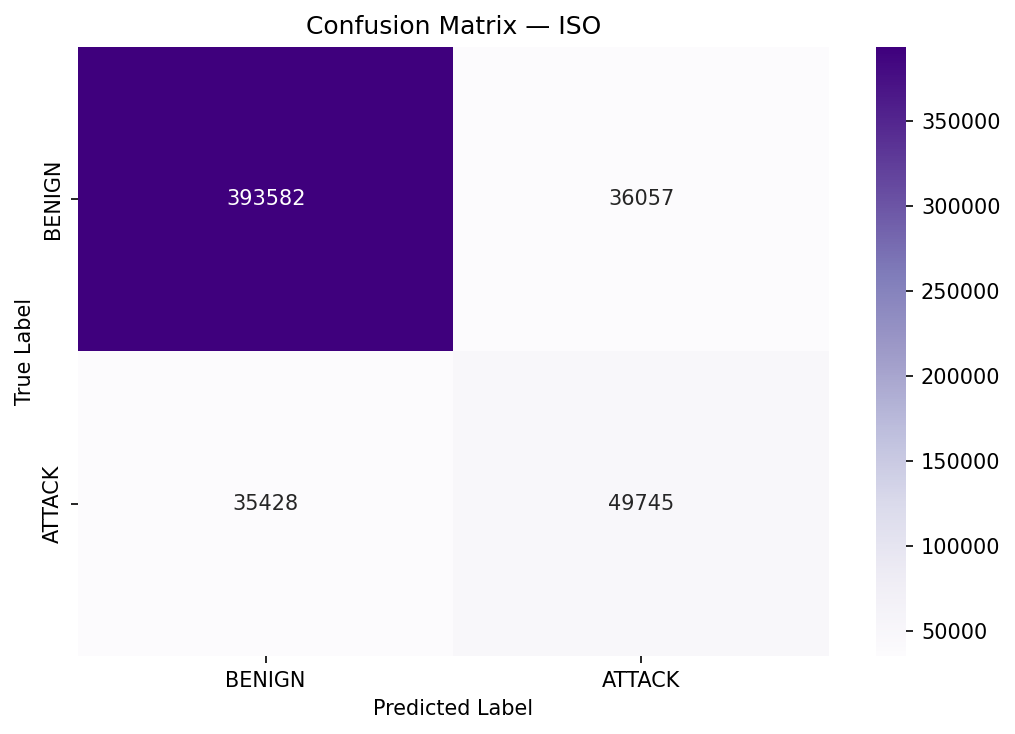
\includegraphics[width=0.80\textwidth]{results/confusion_matrix_iso.png}
\caption{Confusion Matrix for Isolation Forest.}
\label{fig:cm_iso}
\end{figure}

\begin{figure}[H]
\centering
\begin{subfigure}[b]{0.49\textwidth}
    \centering
    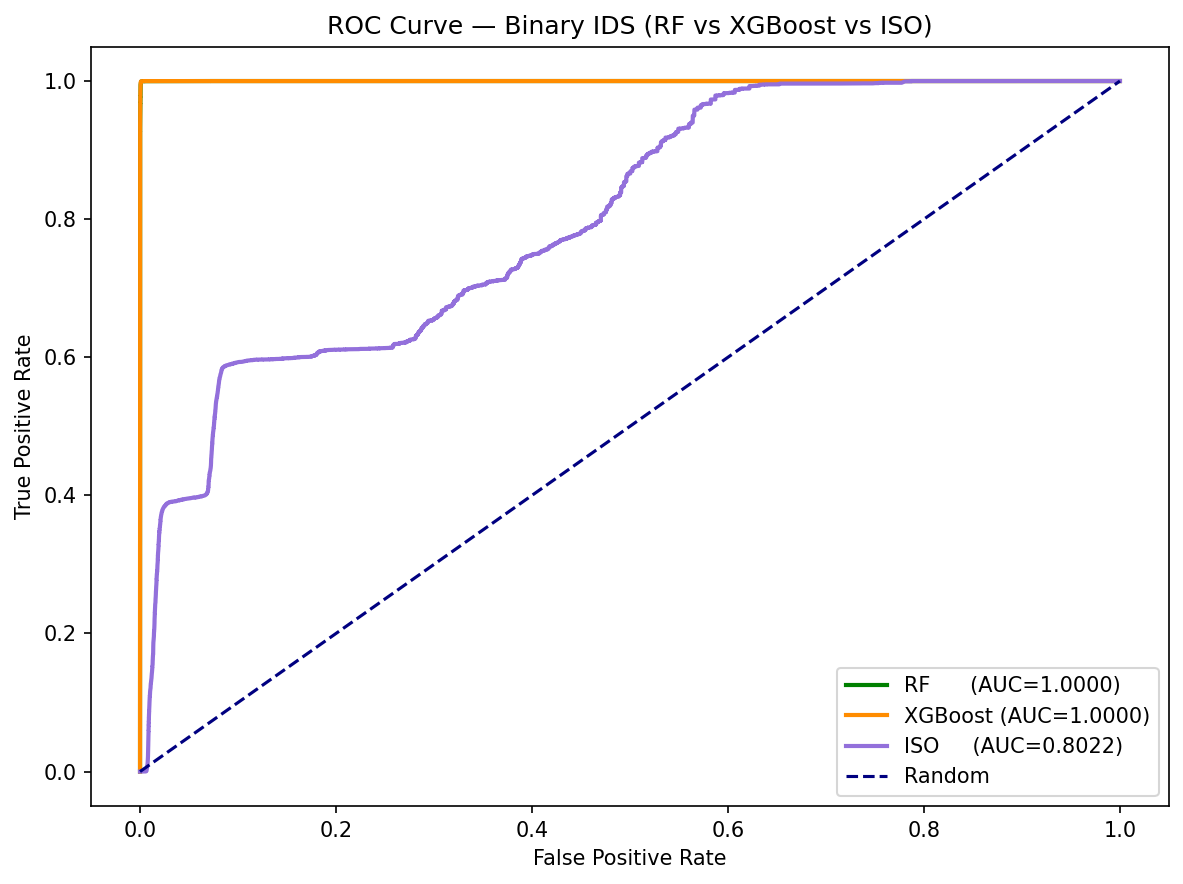
\includegraphics[width=\textwidth]{results/roc_curve.png}
    \caption{ROC Curves.}
    \label{fig:roc}
\end{subfigure}
\hfill
\begin{subfigure}[b]{0.49\textwidth}
    \centering
    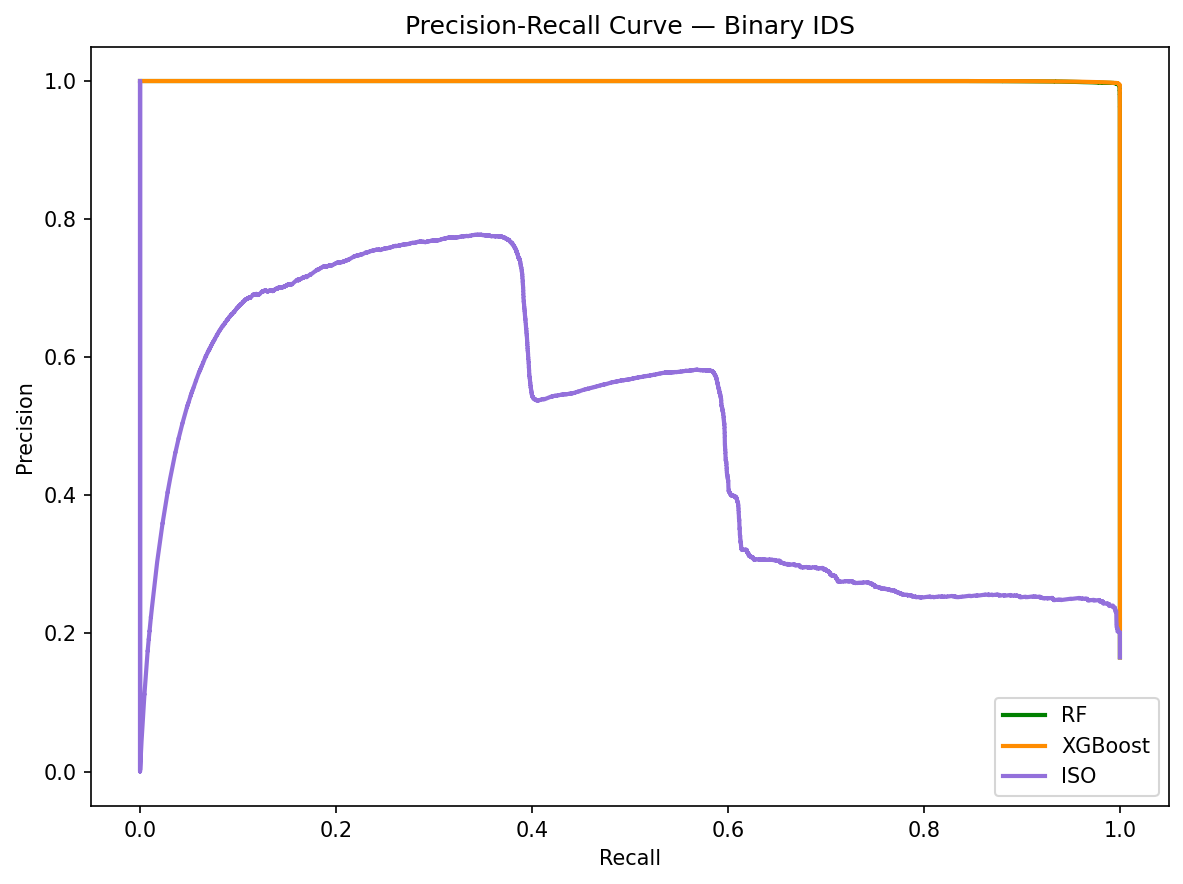
\includegraphics[width=\textwidth]{results/pr_curve.png}
    \caption{PR Curves.}
    \label{fig:pr}
\end{subfigure}
\caption{ROC and Precision-Recall Curves for all models.}
\label{fig:roc_pr}
\end{figure}

\subsection{Multiclass Classification Results}

\subsubsection{Overall Performance}

\begin{table}[H]
\centering
\caption{Multiclass Classification Overall Performance}
\label{tab:multiclass_overall}
\begin{tabular}{|l|r|}
\hline
\textbf{Metric} & \textbf{Value} \\
\hline
Overall Accuracy & 99.84\% \\
Macro Precision & 82.18\% \\
Macro Recall & 91.10\% \\
Macro F1 & 85.07\% \\
Weighted Precision & 99.86\% \\
Weighted Recall & 99.84\% \\
Weighted F1 & 99.85\% \\
\hline
\end{tabular}
\end{table}

\subsubsection{Per-Class Performance}

\begin{table}[H]
\centering
\caption{Per-Class Multiclass Performance}
\label{tab:per_class_results}
\begin{tabular}{|l|r|r|r|r|}
\hline
\textbf{Class} & \textbf{Support} & \textbf{Precision} & \textbf{Recall} & \textbf{F1-Score} \\
\hline
BENIGN & 429,639 & 0.99997 & 0.9986 & 0.9993 \\
DoS Hulk & 34,570 & 0.9979 & 0.9994 & 0.9987 \\
DDoS & 25,603 & 0.9989 & 1.0000 & 0.9994 \\
PortScan & 18,164 & 0.9875 & 0.9993 & 0.9934 \\
DoS GoldenEye & 2,056 & 0.9866 & 0.9995 & 0.9930 \\
FTP-Patator & 1,187 & 0.9983 & 1.0000 & 0.9992 \\
DoS slowloris & 1,075 & 0.9780 & 0.9916 & 0.9848 \\
DoS Slowhttptest & 1,046 & 0.9719 & 0.9904 & 0.9811 \\
SSH-Patator & 644 & 1.0000 & 1.0000 & 1.0000 \\
Bot & 391 & 0.6533 & 0.9974 & 0.7895 \\
Web Attack - BF & 294 & 0.7500 & 0.7551 & 0.7525 \\
Web Attack - XSS & 130 & 0.3961 & 0.4692 & 0.4296 \\
Infiltration & 7 & 0.8333 & 0.7143 & 0.7692 \\
Web Attack - Sql Injection & 4 & 0.3750 & 0.7500 & 0.5000 \\
Heartbleed & 2 & 0.4000 & 1.0000 & 0.5714 \\
\hline
\end{tabular}
\end{table}

\begin{figure}[H]
\centering
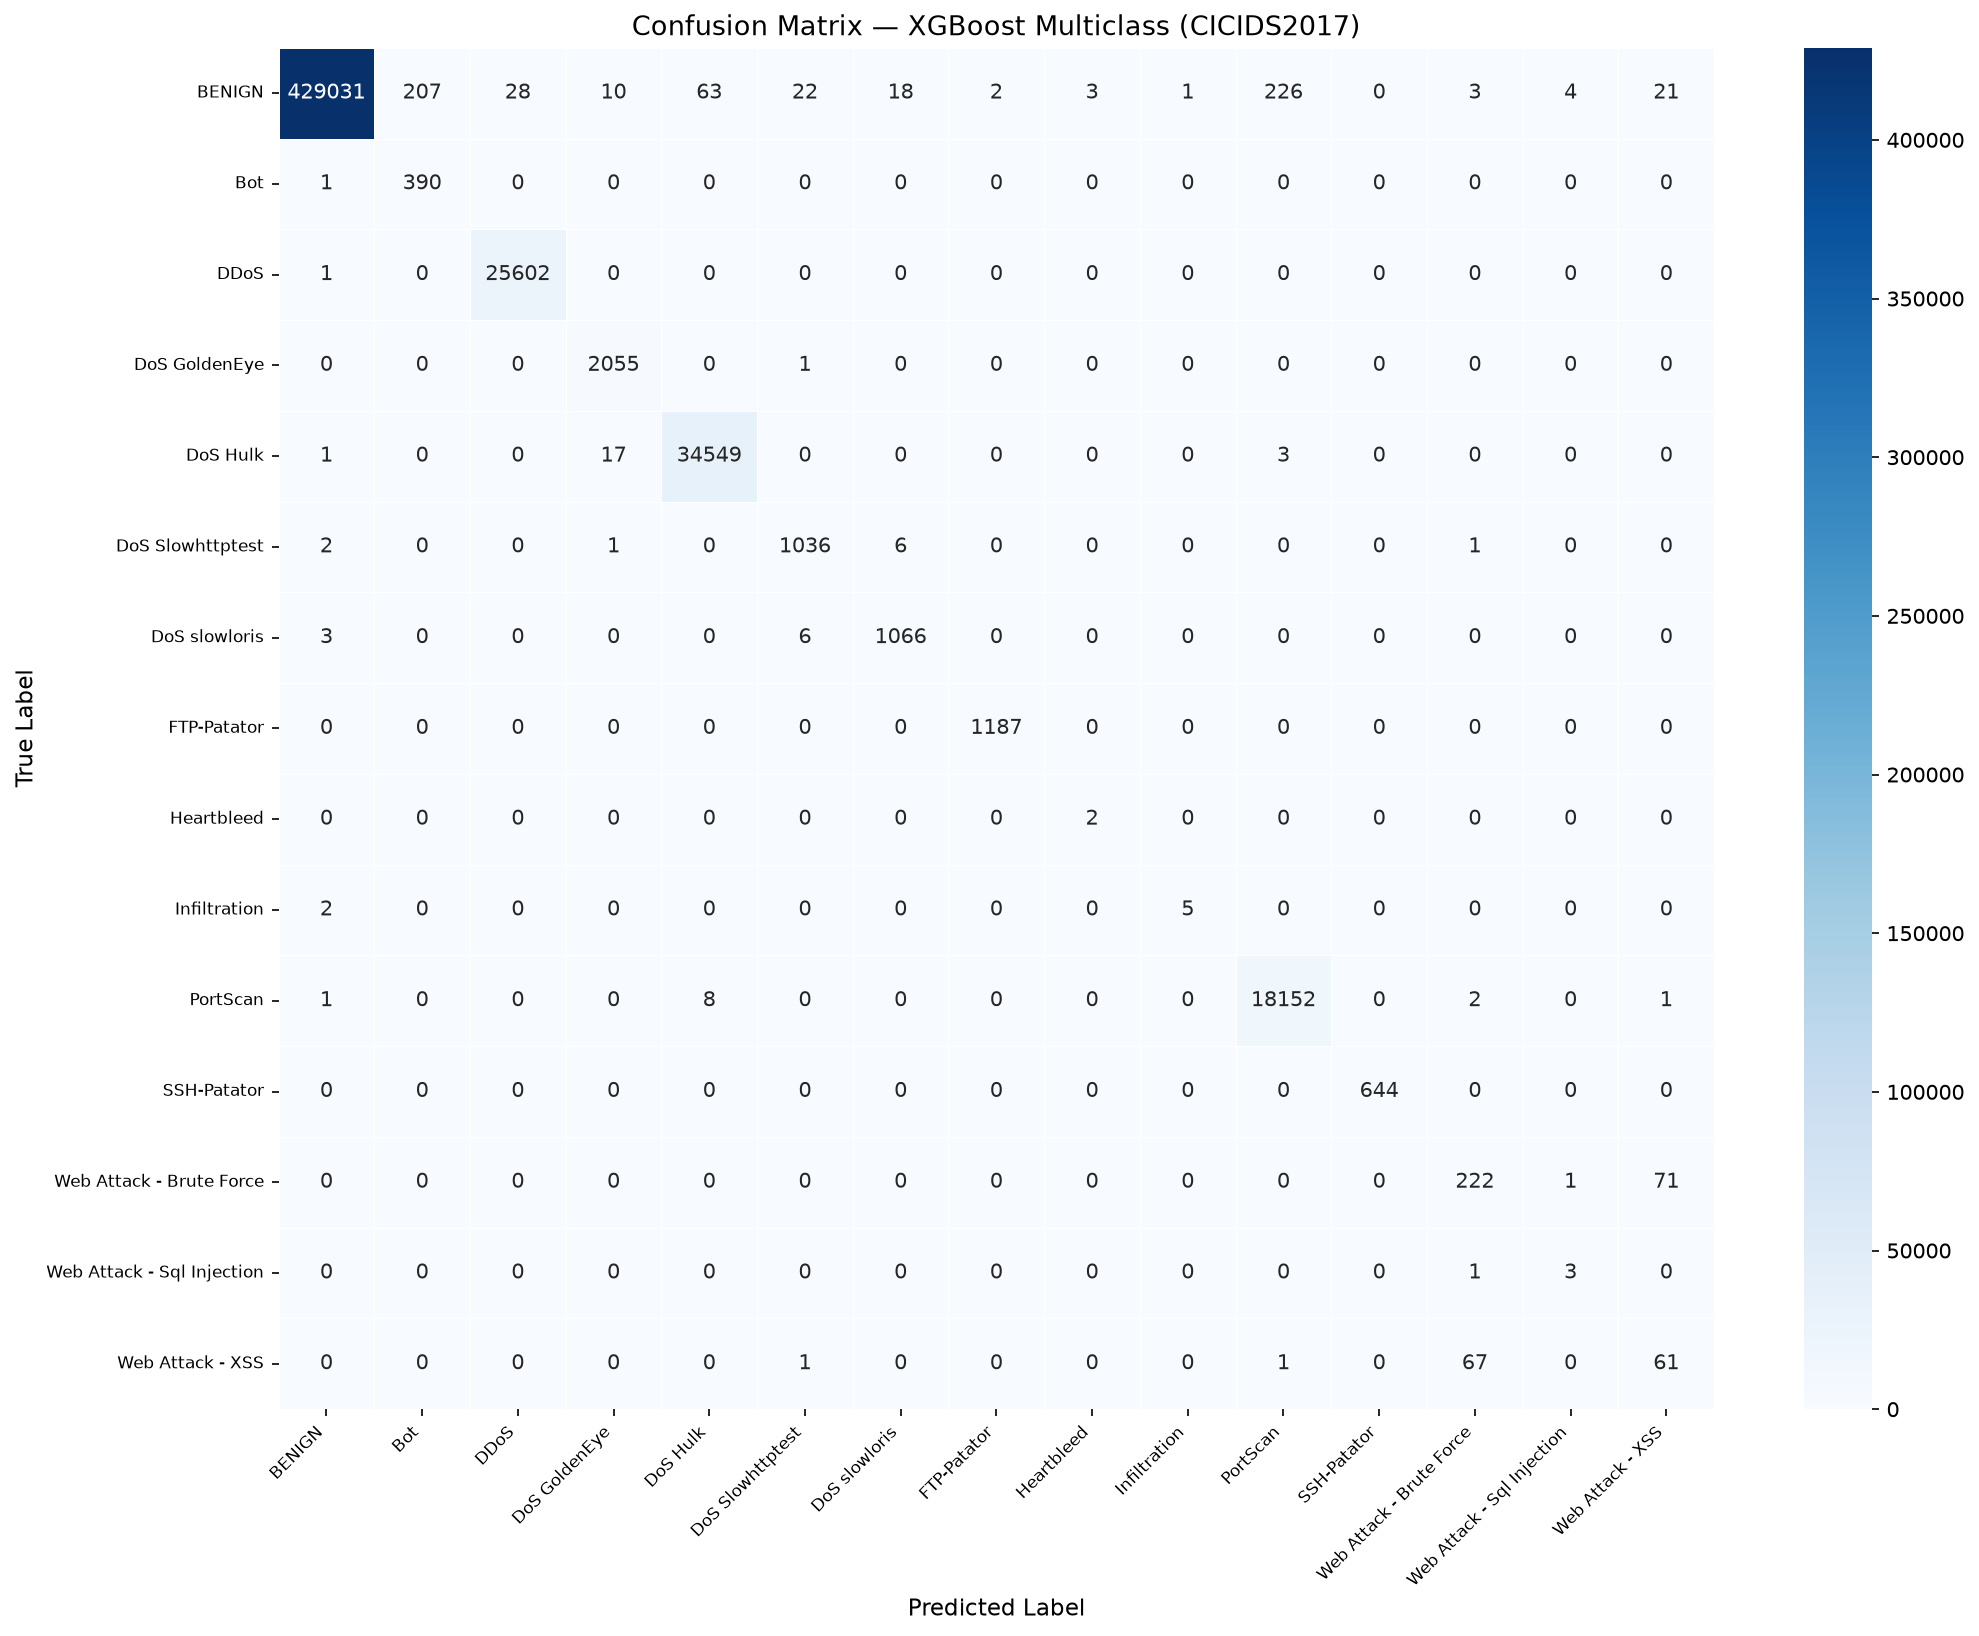
\includegraphics[width=\textwidth]{results/confusion_matrix_multiclass.png}
\caption{Confusion Matrix for XGBoost Multiclass Classifier.}
\label{fig:cm_multiclass}
\end{figure}

The multiclass confusion matrix (Figure~\ref{fig:cm_multiclass}) illustrates the exact breakdown of predicted vs. true labels across 15 traffic categories. 
\begin{itemize}
    \item \textbf{Diagonal Concentration}: The matrix exhibits a dominant main diagonal ($X=Y$), confirming that the vast majority of test samples are correctly classified. For example, 429,031 out of 429,639 BENIGN flows ($99.86\%$), 25,602 out of 25,603 DDoS flows ($100.00\%$), 34,549 out of 34,570 DoS Hulk flows ($99.94\%$), and 18,152 out of 18,164 PortScan flows ($99.93\%$) are correctly assigned.
    \item \textbf{Behavioral Confusions}: Minor misclassifications off the diagonal occur almost exclusively between attack types sharing similar network flow statistics, such as Web Attack--Brute Force vs. XSS (71 samples confused due to identical HTTP POST metadata), SlowHTTPTest vs. Slowloris, and DoS GoldenEye vs. DoS Hulk.
    \item \textbf{Dual-Stage Complementarity}: Stage 1 (Binary XGBoost) resolves \textit{"Is this flow an attack?"} (`BENIGN` vs. `ATTACK`) at high throughput, while Stage 2 (Multiclass XGBoost) answers \textit{"What specific attack category is present?"} to drive contextual mitigation.
\end{itemize}

\subsection{Real-Time Performance Results}

\begin{table}[H]
\centering
\caption{Real-Time Inference Performance (Single-thread)}
\label{tab:runtime_performance}
\begin{tabular}{|l|r|r|r|}
\hline
\textbf{Metric} & \textbf{BENIGN Path} & \textbf{ATTACK Path} & \textbf{Overall} \\
\hline
Avg Latency & 4.73 ms & 6.82 ms & 5.08 ms \\
P50 Latency & 4.52 ms & 6.51 ms & - \\
P95 Latency & 7.83 ms & 11.28 ms & - \\
P99 Latency & 10.95 ms & 14.87 ms & - \\
Throughput & 211 pred/s & 147 pred/s & 197 pred/s \\
\hline
\end{tabular}
\end{table}

\subsection{Inference Speed Comparison}

To justify the selection of XGBoost over alternatives, Table~\ref{tab:inference_speed} compares inference latency, throughput, and model size.

\begin{table}[H]
\centering
\caption{Inference Speed Comparison across Models}
\label{tab:inference_speed}
\begin{tabular}{|l|r|r|r|}
\hline
\textbf{Model} & \textbf{Avg Latency (ms)} & \textbf{Throughput (pred/s)} & \textbf{Model Size (MB)} \\
\hline
Random Forest (Binary) & $\sim$12.5 & $\sim$80 & 76.10 \\
Isolation Forest & $\sim$3.2 & $\sim$310 & 1.42 \\
XGBoost (Binary + Multi) & 5.08 & 197 & 10.16 \\
\hline
\end{tabular}
\end{table}

XGBoost achieves the best balance: high accuracy (99.74\% F1), low latency, and a compact model size, making it ideal for deployment.

\subsection{Feature Importance Analysis}

\begin{table}[H]
\centering
\caption{Top 10 Feature Importances (XGBoost Multiclass)}
\label{tab:feature_importance}
\begin{tabular}{|l|r|}
\hline
\textbf{Feature} & \textbf{Importance} \\
\hline
Average Packet Size & 0.2693 \\
Bwd Packet Length Std & 0.2239 \\
Avg Bwd Segment Size & 0.0911 \\
Bwd Header Length & 0.0865 \\
Max Packet Length & 0.0514 \\
Bwd Packet Length Mean & 0.0513 \\
Fwd Packet Length Max & 0.0341 \\
Active Std & 0.0199 \\
FIN Flag Count & 0.0157 \\
Fwd Header Length.1 & 0.0128 \\
\hline
\end{tabular}
\end{table}

\begin{figure}[H]
\centering
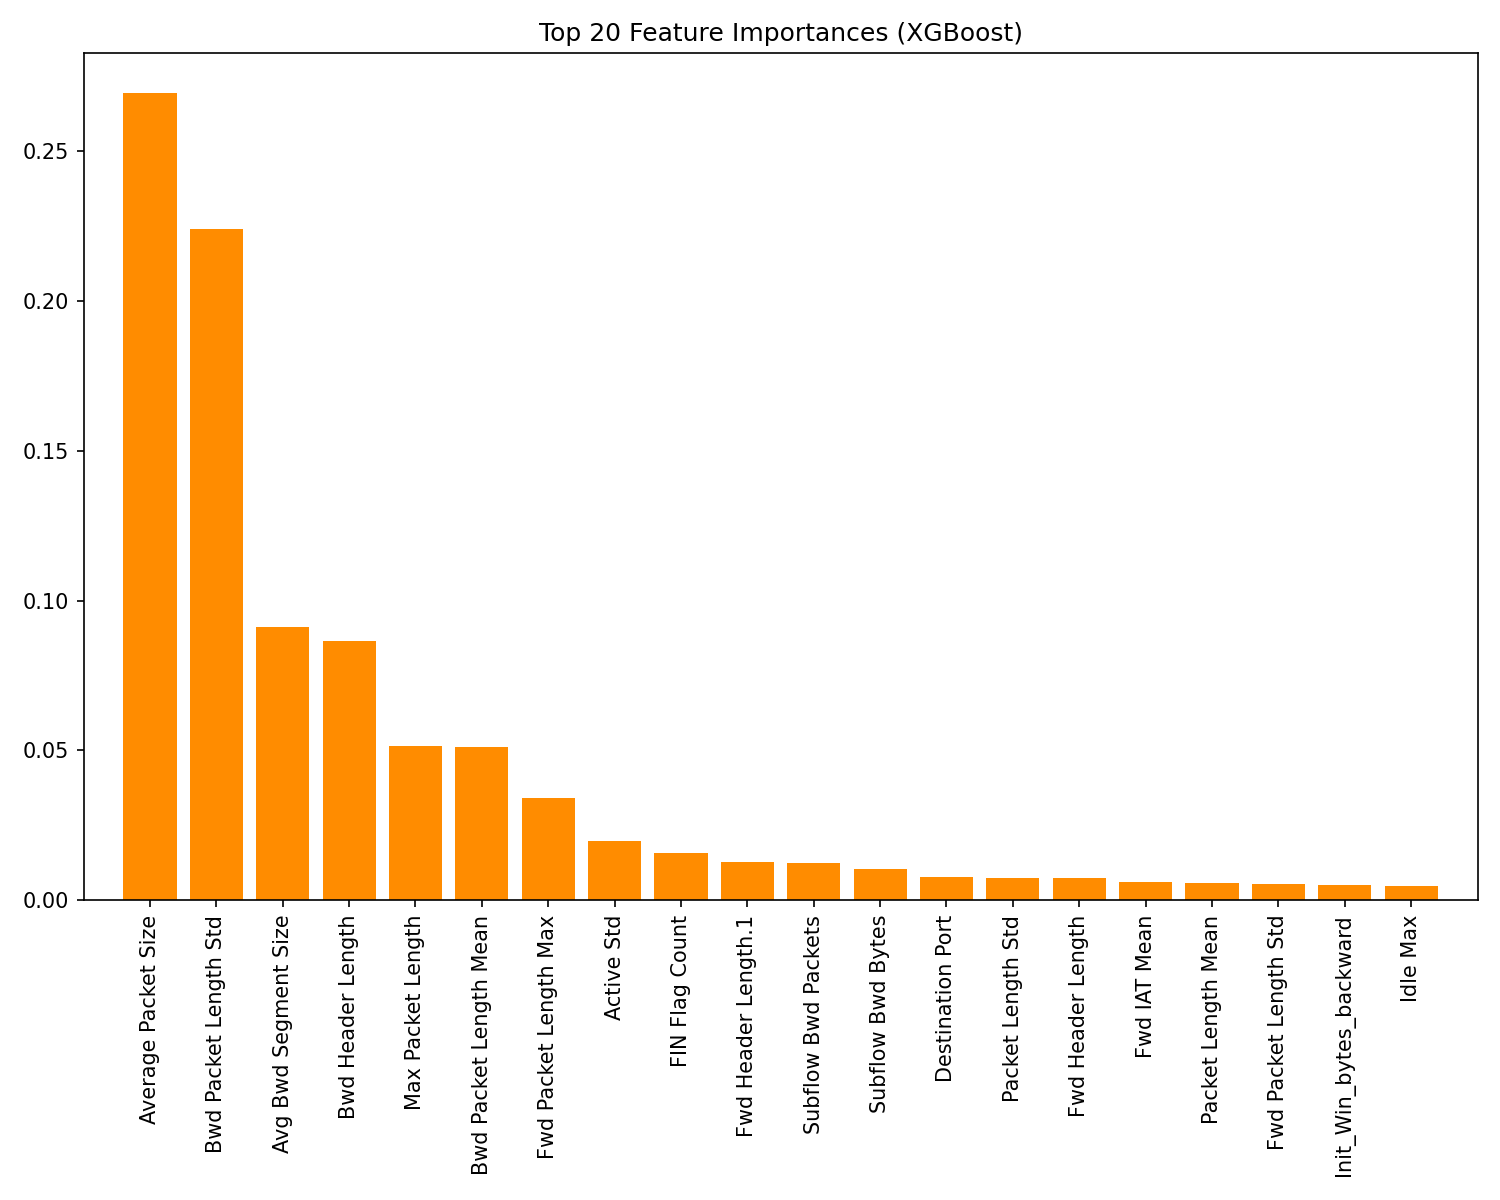
\includegraphics[width=\textwidth]{results/xgb_feature_importance.png}
\caption{Top 20 Feature Importances for XGBoost Binary.}
\label{fig:fi_xgb}
\end{figure}

\begin{figure}[H]
\centering
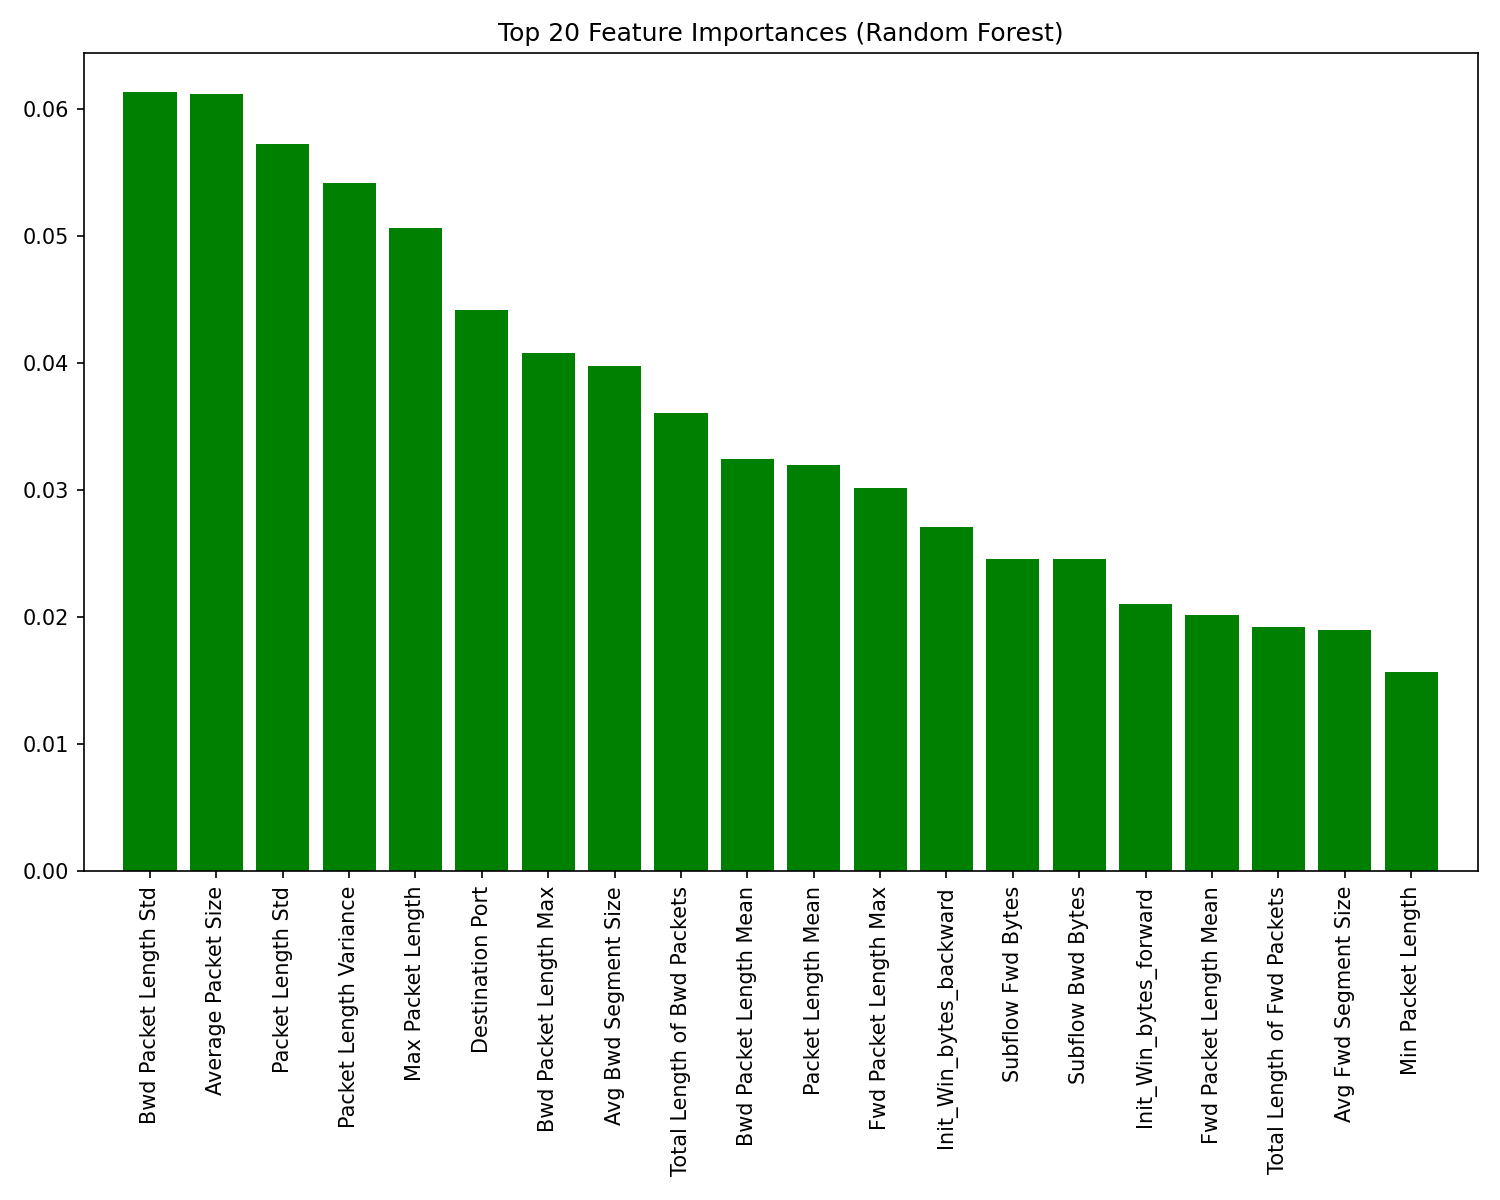
\includegraphics[width=\textwidth]{results/rf_feature_importance.png}
\caption{Top 20 Feature Importances for Random Forest Binary.}
\label{fig:fi_rf}
\end{figure}

\begin{figure}[H]
\centering
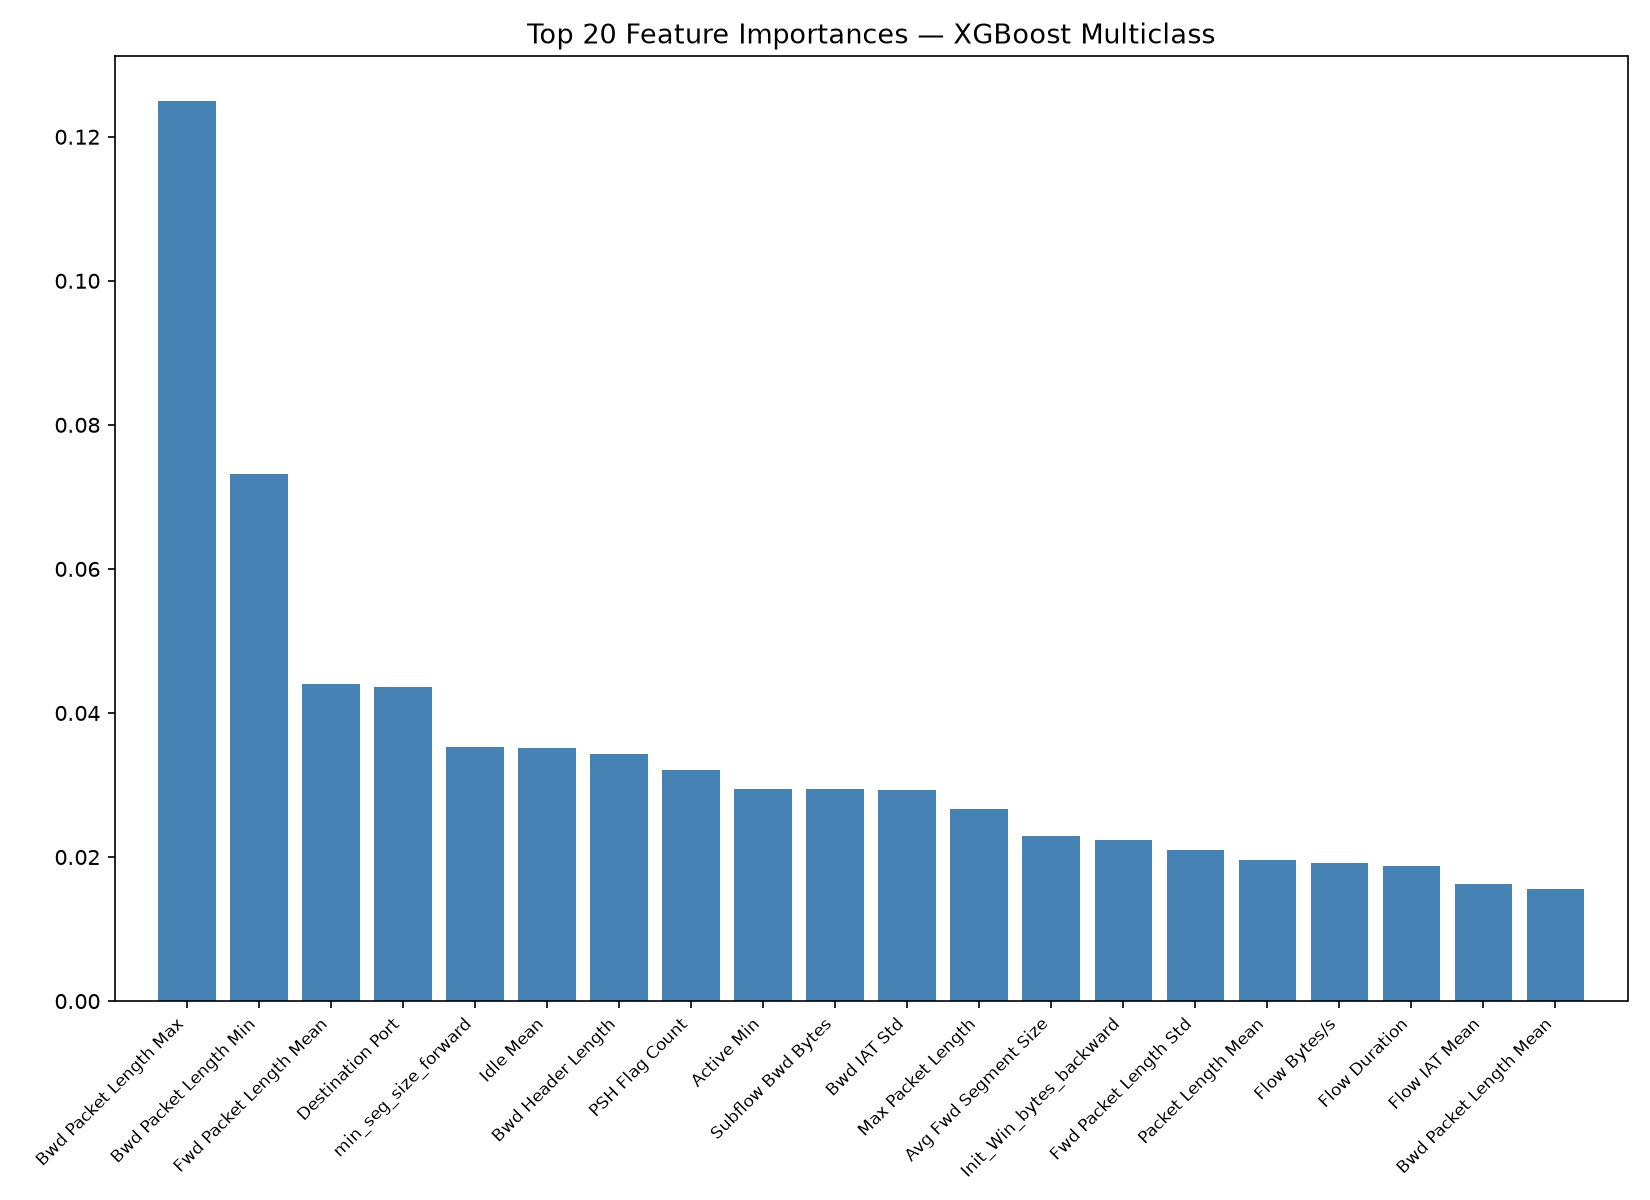
\includegraphics[width=\textwidth]{results/feature_importance_multiclass.png}
\caption{Top 20 Feature Importances for XGBoost Multiclass.}
\label{fig:fi_multiclass}
\end{figure}

\subsection{Model Size Analysis}

\begin{table}[H]
\centering
\caption{Model File Sizes}
\label{tab:model_sizes}
\begin{tabular}{|l|r|}
\hline
\textbf{Model File} & \textbf{Size (MB)} \\
\hline
xgb\_binary.pkl & 1.47 \\
xgb\_multiclass.pkl & 8.69 \\
rf\_binary.pkl & 76.10 \\
isolation\_forest.pkl & 1.42 \\
\hline
\textbf{Total (XGBoost + IF)} & \textbf{11.58 MB} \\
\hline
\end{tabular}
\end{table}

% ============================================================================
% SECTION 8: DISCUSSION
% ============================================================================
\section{Discussion}

\subsection{Interpretation of Results}

The experimental results demonstrate the effectiveness of the proposed AI-RTIDS system:

\begin{enumerate}
    \item \textbf{High Detection Accuracy}: XGBoost achieves precision 99.68\%, recall 99.81\%, and F1 99.74\% on 514,812 test samples.
    \item \textbf{Real-Time Capability}: 5.08 ms average latency and 197 predictions/sec (single-thread, experimentally measured); projected $\sim$2700 flows/sec with 14-worker scaling.
    \item \textbf{Resource Efficiency}: 11.58 MB total model size enables deployment on resource-constrained hardware.
    \item \textbf{Anomaly Detection}: Isolation Forest provides zero-day capability with composite severity scoring:
    \begin{equation}
        S = 0.65 \times p_{\text{attack}} + 0.35 \times s_{\text{iso}}
        \label{eq:severity}
    \end{equation}
    where $p_{\text{attack}} \in [0,1]$ is the binary XGBoost probability and $s_{\text{iso}} \in [0,1]$ is the normalised Isolation Forest anomaly score. The composite score $S$ is mapped to severity levels: CRITICAL ($S \geq 0.90$), HIGH ($S \geq 0.75$), MEDIUM ($S \geq 0.55$), LOW ($S \geq 0.35$), NONE ($S < 0.35$).
\end{enumerate}

\subsection{Rare Class Performance}

Minority classes (Heartbleed, SQL Injection, XSS) show lower F1 scores due to extreme class imbalance (as few as 11 samples). This is a known limitation of CIC-IDS-2017.

\subsection{Comparison with Reference Paper}

\begin{table}[H]
\centering
\caption{Comparison with Alromaihi et al. \cite{alromaihi2025design}}
\label{tab:reference_comparison}
\begin{tabular}{|p{3cm}|p{4cm}|p{4cm}|}
\hline
\textbf{Aspect} & \textbf{Reference Paper} & \textbf{Proposed AI-RTIDS} \\
\hline
Best Model & XGBoost & XGBoost \\
CIC-IDS-2017 Accuracy & 99.84\% & 99.84\% \\
Attack Classes & Binary & 15 multiclass \\
Anomaly Detection & Not implemented & Isolation Forest \\
Alert Deduplication & Not implemented & 60-second window \\
SQLite Persistence & Not implemented & Implemented \\
Prometheus Metrics & Not implemented & Implemented \\
Real-Time Performance & Not reported & 5.08 ms, 197 pred/s \\
Model Size & Not reported & 11.58 MB \\
\hline
\end{tabular}
\end{table}

\subsection{Advantages}
\begin{enumerate}
    \item Comprehensive 15-class attack coverage.
    \item Small total model size (11.58 MB).
    \item Dual-stage pipeline optimizes throughput via early exit.
    \item Production-ready design with Prometheus, SQLite, and Docker Compose.
    \item Configurable alert deduplication and rule filtering.
    \item Optional REST/WebSocket API for integration.
\end{enumerate}

\subsection{Limitations}
\begin{enumerate}
    \item Dataset bias (trained on CIC-IDS-2017 only).
    \item Rare class performance constrained by data scarcity.
    \item No payload analysis (encrypted traffic).
    \item Not yet validated in a live production environment.
    \item Default threshold (0.50) requires per-network tuning.
\end{enumerate}

\subsection{Threat Model and Assumptions}

The proposed IDS operates under the following assumptions:
\begin{itemize}
    \item The network traffic is captured from a single point (e.g., a mirror port or network tap) and is assumed to be a complete representation of all traffic.
    \item The system is deployed in a trusted environment where the capture device and the IDS host are not compromised.
    \item The attack patterns are represented in the CIC-IDS-2017 dataset; zero-day attacks are handled by the Isolation Forest, which is trained on benign traffic only.
    \item The system is designed for detection, not prevention; it raises alerts for security analysts to respond.
\end{itemize}
Future work will consider adversarial evasion and model poisoning.

\subsection{Security and Robustness}
The system includes thread-safe flow management, graceful shutdown, median imputation, and bounded flow table size. Potential adversarial evasion and training data poisoning are noted as future research directions.

\subsection{Ethical Considerations}
The AI-RTIDS is designed exclusively for defensive security. CIC-IDS-2017 contains no PII. All experiments were conducted in a controlled environment.

% ============================================================================
% SECTION 9: CONCLUSIONS AND FUTURE WORK
% ============================================================================
\section{Conclusions and Future Work}

\subsection{Summary of Contributions}

This project presented a complete AI-Driven Real-Time Intrusion Detection System:

\begin{enumerate}
    \item Dual-stage detection pipeline (Binary XGBoost $\rightarrow$ Multiclass XGBoost + Isolation Forest).
    \item Fully functional implementation with packet capture, flow management, feature extraction, inference, alerting, and SQLite persistence.
    \item 15-class attack identification with 99.84\% overall accuracy.
    \item Real-time performance: 5.08 ms latency, 197 pred/sec (single-thread, experimentally measured), projected $\sim$2700 flows/sec with multi-worker scaling.
    \item 11.58 MB total model size suitable for edge deployment.
    \item Integrated monitoring stack (Prometheus, Grafana) and REST/WebSocket API (FastAPI).
\end{enumerate}

\subsection{Key Findings}
\begin{enumerate}
    \item XGBoost achieves competitive detection accuracy (99.74\% F1) with minimal resource usage.
    \item Dual-stage pipeline effectively reduces computational overhead.
    \item Isolation Forest provides complementary zero-day detection.
    \item Alert deduplication prevents alert flooding.
\end{enumerate}

\subsection{Future Work}
\label{sec:future_work}

The following enhancements are organised by implementation priority based on their impact on operational security, integration readiness, and deployment value. All items listed below are \textbf{not yet implemented} in the current system.

\subsubsection{Priority 1 — Alert Manager Enhancements (High Impact, Low Effort)}

The existing \texttt{AlertManager} provides rule filtering, deduplication, and SQLite persistence but lacks real-time operator notification. The following extensions can be plugged directly into the \texttt{process()} method without architectural changes:

\begin{enumerate}
    \item \textbf{Severity-Based Alert Routing}: Route CRITICAL and HIGH alerts to a fast-path notification channel (e.g. immediate push notification) while queuing MEDIUM/LOW alerts for batched delivery. Requires a priority queue between the alert manager and notification senders.

    \item \textbf{Email Notification} (SMTP): Send formatted alert summaries for CRITICAL severity events using Python's built-in \texttt{smtplib}. Configuration (SMTP host, port, credentials, recipients) stored in \texttt{config.json}. Throttling should mirror the existing deduplication window to prevent inbox flooding.

    \item \textbf{Slack Webhook Notification}: Post alert cards to a Slack channel via the Slack Incoming Webhooks API (HTTP POST with JSON payload). The card should include attack type, severity, src/dst IP, and timestamp. A single HTTPS call per unique alert; deduplication window prevents duplicate messages.

    \item \textbf{Telegram Bot Notification}: Send alert messages to a Telegram chat via the Bot API (\texttt{sendMessage} endpoint). Lightweight, free, and does not require server-side infrastructure. Suitable for individual analyst or on-call team notifications.

    \item \textbf{Generic Webhook Support}: Accept a list of user-configured HTTPS endpoints in \texttt{config.json} and POST a standardised JSON payload (matching the \texttt{PredictionResult} schema) to each registered URL. This enables integration with any third-party system (PagerDuty, OpsGenie, custom SIEM ingestion endpoints) without modifying the IDS core.
\end{enumerate}

\subsubsection{Priority 2 — Severity Scoring Improvements (Medium Impact)}

The current composite severity formula $S = 0.65 \times p_{\text{attack}} + 0.35 \times s_{\text{iso}}$ uses static weights derived empirically during development. The following improvements would make severity scoring more reliable in production:

\begin{enumerate}
    \item \textbf{Per-Attack-Type Severity Weights}: Assign higher base severity to inherently dangerous attack types (e.g. Heartbleed, SQL Injection) regardless of XGBoost probability, since these attack classes have very few training samples and may underestimate their actual risk.

    \item \textbf{Temporal Severity Escalation}: Escalate the severity of repeated attacks from the same source IP over time. If the same (src\_ip, attack\_type) tuple triggers three consecutive MEDIUM alerts within five minutes, escalate to HIGH automatically.

    \item \textbf{Calibrated Probability Output}: Apply Platt scaling or isotonic regression to calibrate XGBoost output probabilities so that $p_{\text{attack}} = 0.80$ reliably reflects an 80\% empirical attack rate on held-out data. This makes the composite score more interpretable.

    \item \textbf{Network-Adaptive Threshold Tuning}: Implement an automated threshold selection routine that monitors live false-positive and false-negative rates over a rolling window and adjusts \texttt{binary\_threshold} in \texttt{config.json} without requiring a full model retrain.
\end{enumerate}

\subsubsection{Priority 3 — Deduplication Enhancements (Medium Impact)}

The current deduplication mechanism suppresses repeated (src\_ip, dst\_ip, attack\_type) tuples within a fixed 60-second window. The following improvements address edge cases:

\begin{enumerate}
    \item \textbf{Subnet-Level Deduplication}: Group alerts by source subnet (e.g. /24) rather than individual IP address to suppress distributed scanning campaigns that rotate source IPs while targeting the same subnet.

    \item \textbf{Attack-Class-Specific Windows}: Apply shorter dedup windows for rapidly evolving attacks (e.g. 10 seconds for DDoS) and longer windows for slow attacks (e.g. 300 seconds for Infiltration), rather than a single global window.

    \item \textbf{Dedup Cache Persistence}: Persist the deduplication cache to SQLite on shutdown and reload it on startup. Without this, a process restart resets the cache and may produce a burst of duplicate alerts for ongoing attacks.

    \item \textbf{Dedup Cache Size Bounding}: Cap the in-memory dedup cache at a configurable maximum entry count (e.g. 100,000 entries) with LRU eviction to prevent unbounded memory growth under sustained DDoS conditions.
\end{enumerate}

\subsubsection{Priority 4 — Medium-Term Research Directions}

\begin{enumerate}
    \item \textbf{Multi-Dataset Validation}: Evaluate on UNSW-NB15, CSE-CIC-IDS2018, and NF-ToN-IoT to assess cross-domain generalisation.
    \item \textbf{Encrypted Traffic Analysis}: Integrate JA3/JA3S TLS fingerprinting for behavioural classification without payload decryption.
    \item \textbf{MITRE ATT\&CK Mapping}: Map detected attack types to MITRE ATT\&CK tactics and techniques to produce industry-standard threat reports.
    \item \textbf{SIEM Integration}: Forward structured alerts to Splunk, Elastic SIEM, or IBM QRadar via syslog or Kafka.
    \item \textbf{Rate Limiting and Back-Pressure}: Add per-interface packet drop counters and adaptive flow export throttling to prevent RAM exhaustion under sustained high-volume attacks.
\end{enumerate}

\subsubsection{Priority 5 — Long-Term Vision}

\begin{enumerate}
    \item Federated learning for privacy-preserving model updates across multiple organisations.
    \item Threat intelligence integration for automatic blocklist updates from detected malicious IPs.
    \item Kubernetes-based horizontal scaling for high-throughput enterprise deployment.
    \item Deep learning exploration (LSTM, Transformer) for sequence-based attack detection.
    \item Adversarial robustness: defences against evasion attacks and model poisoning.
\end{enumerate}

% ============================================================================
% REFERENCES
% ============================================================================
\begin{thebibliography}{99}

\bibitem{ahmad2021network}
Ahmad, Z.; Shahid Khan, A.; Wai Shiang, C.; Abdullah, J.; Ahmad, F. (2021).
Network intrusion detection system: A systematic study of machine learning and deep learning approaches.
\textit{Transactions on Emerging Telecommunications Technologies}, 32(8), e4150.

\bibitem{attou2023cloud}
Attou, H.; Guezza, A.; Benkirane, S.; Azrour, M.; Farhaoui, Y. (2023).
Cloud-Based Intrusion Detection Approach Using Machine Learning Techniques.
\textit{Big Data Mining and Analytics}, 6, 311-320.

\bibitem{saheed2022machine}
Saheed, Y.K.; Abiodun, A.I.; Misra, S.; Holone, M.K.; Colomo-Palacios, R. (2022).
A machine learning-based intrusion detection for detecting internet of things network attacks.
\textit{Alexandria Engineering Journal}, 61, 9395-9409.

\bibitem{seth2021novel}
Seth, S.; Singh, G.; Kaur Chahal, K. (2021).
A novel time efficient learning-based approach for smart intrusion detection system.
\textit{Journal of Big Data}, 8, 111.

\bibitem{talukder2023dependable}
Talukder, M.A.; Hasan, K.F.; Islam, M.M.; Uddin, M.A.; Akhter, A.; Yousuf, M.A.; Alharbi, F.; Moni, M.A. (2023).
A dependable hybrid machine learning model for network intrusion detection.
\textit{Journal of Information Security and Applications}, 72, 103405.

\bibitem{hnamte2023dcnnbilstm}
Hnamte, V.; Hussain, J. (2023).
DCNNBiLSTM: An Efficient Hybrid Deep Learning-Based Intrusion Detection System.
\textit{Telematics and Informatics Reports}, 10, 100053.

\bibitem{alromaihi2025design}
Alromaihi, N.; Rouached, M.; Akremi, A. (2025).
Design and Analysis of an Effective Architecture for Machine Learning Based Intrusion Detection Systems.
\textit{Network}, 5(2), 13.

\bibitem{sharafaldin2018toward}
Sharafaldin, I.; Lashkari, A.H.; Ghorbani, A.A. (2018).
Toward generating a new intrusion detection dataset and intrusion traffic characterization.
\textit{Proceedings of the 4th International Conference on Information Systems Security and Privacy (ICISSP)}, 108-116.

\bibitem{verma2020machine}
Verma, A.; Ranga, V. (2020).
Machine learning based intrusion detection systems for IoT applications.
\textit{Wireless Personal Communications}, 111, 2287-2310.

\bibitem{li2019machine}
Li, J.; Qu, Y.; Chao, F.; Shum, H.P.; Ho, E.S.; Yang, L. (2019).
Machine learning algorithms for network intrusion detection.
\textit{AI in Cybersecurity}, 151-179.

\bibitem{axelson2000intrusion}
Axelsson, S. (2000).
Intrusion Detection Systems: A Survey and Taxonomy.
\textit{Technical Report 99-15}, Chalmers University.

\bibitem{garcia2009anomaly}
Garcia-Teodoro, P.; Diaz-Verdejo, J.; Macia-Fernandez, G.; Vazquez, E. (2009).
Anomaly-based network intrusion detection: Techniques, systems and challenges.
\textit{Computers \& Security}, 28(1-2), 18-28.

\bibitem{zhang2019network}
Zhang, J.; Zulkernine, M.; Haque, A. (2019).
Random-forests-based network intrusion detection systems.
\textit{IEEE Transactions on Systems, Man, and Cybernetics}, 38(5), 649-659.

\bibitem{thakkar2018survey}
Thakkar, A.; Lohiya, R. (2018).
A survey on intrusion detection system: feature selection, model, performance measures, application perspective, challenges, and future research directions.
\textit{Artificial Intelligence Review}, 55, 453-563.

\bibitem{larabi2019machine}
Larabi, M.; Lehsaini, M.; Lounis, A. (2019).
Machine learning for network intrusion detection: A comparative study.
\textit{IEEE Access}, 7, 155276-155290.

\bibitem{fernandes2019comprehensive}
Fernandes, G.; Carvalho, L.; Rodrigues, J. (2019).
A comprehensive review of intrusion detection systems.
\textit{IEEE Communications Surveys \& Tutorials}, 21(3), 2356-2386.

\bibitem{chen2016xgboost}
Chen, T.; Guestrin, C. (2016).
XGBoost: A scalable tree boosting system.
\textit{Proceedings of the 22nd ACM SIGKDD International Conference on Knowledge Discovery and Data Mining}, 785-794.

\bibitem{he2009learning}
He, H.; Garcia, E. A. (2009).
Learning from imbalanced data.
\textit{IEEE Transactions on Knowledge and Data Engineering}, 21(9), 1263-1284.

\bibitem{lashkari2018cse}
Lashkari, A. H.; Draper-Gil, G.; Mamun, M. S. I.; Ghorbani, A. A. (2018).
Characterization of encrypted and VPN traffic using time-related features.
\textit{Proceedings of the 2nd International Conference on Information Systems Security and Privacy}, 407-414.

\end{thebibliography}

% ============================================================================
% APPENDICES
% ============================================================================
\appendix

\section{Attack Class Descriptions}
\begin{longtable}{|p{3cm}|p{8cm}|}
\caption{Attack Class Descriptions}
\label{app:attack_classes}\\
\hline
\textbf{Attack Type} & \textbf{Description} \\
\hline
\endfirsthead
\multicolumn{2}{c}%
{{\bfseries \tablename\ \thetable{} -- continued}} \\
\hline
\textbf{Attack Type} & \textbf{Description} \\
\hline
\endhead
\hline
\endlastfoot
BENIGN & Normal network traffic \\
DDoS & Distributed Denial of Service \\
DoS GoldenEye & HTTP-based DoS attack \\
DoS Hulk & HTTP flood DoS attack \\
DoS Slowhttptest & Slow HTTP DoS attack \\
DoS slowloris & Slow TCP connection DoS \\
FTP-Patator & FTP brute force attack \\
SSH-Patator & SSH brute force attack \\
Bot & Botnet command and control traffic \\
Infiltration & Network infiltration \\
PortScan & Port scanning reconnaissance \\
Web Attack - Brute Force & HTTP login brute force \\
Web Attack - XSS & Cross-site scripting attack \\
Web Attack - SQL Injection & SQL injection attack \\
Heartbleed & OpenSSL Heartbleed exploit \\
\hline
\end{longtable}

\section{Model Hyperparameters}
\subsection{XGBoost Binary}
\begin{table}[H]
\centering
\caption{XGBoost Binary Hyperparameters}
\begin{tabular}{|l|l|p{5cm}|}
\hline
\textbf{Parameter} & \textbf{Value} & \textbf{Description} \\
\hline
n\_estimators & 300 & Number of boosting rounds \\
max\_depth & 8 & Maximum tree depth \\
learning\_rate & 0.05 & Step size shrinkage \\
subsample & 0.8 & Fraction of samples per tree \\
colsample\_bytree & 0.8 & Fraction of features per tree \\
scale\_pos\_weight & 5.04 & BENIGN:ATTACK ratio \\
reg\_alpha & 0.5 & L1 regularization \\
reg\_lambda & 1.0 & L2 regularization \\
eval\_metric & logloss & Evaluation metric \\
tree\_method & hist & Histogram-based algorithm \\
\hline
\end{tabular}
\end{table}

\subsection{XGBoost Multiclass}
\begin{table}[H]
\centering
\caption{XGBoost Multiclass Hyperparameters}
\begin{tabular}{|l|l|p{5cm}|}
\hline
\textbf{Parameter} & \textbf{Value} & \textbf{Description} \\
\hline
objective & multi:softprob & Multiclass objective \\
num\_class & 15 & Number of classes \\
n\_estimators & 300 & Number of boosting rounds \\
max\_depth & 6 & Maximum tree depth \\
learning\_rate & 0.05 & Step size shrinkage \\
subsample & 0.8 & Fraction of samples per tree \\
colsample\_bytree & 0.8 & Fraction of features per tree \\
reg\_alpha & 0.5 & L1 regularization \\
reg\_lambda & 1.0 & L2 regularization \\
eval\_metric & mlogloss & Multiclass log loss \\
\hline
\end{tabular}
\end{table}

\subsection{Random Forest Binary}
\begin{table}[H]
\centering
\caption{Random Forest Binary Hyperparameters}
\begin{tabular}{|l|l|p{5cm}|}
\hline
\textbf{Parameter} & \textbf{Value} & \textbf{Description} \\
\hline
n\_estimators & 300 & Number of decision trees in the forest \\
max\_depth & 20 & Maximum depth of each tree \\
min\_samples\_leaf & 2 & Minimum samples required at a leaf node \\
class\_weight & balanced & Handles 5.04:1 BENIGN:ATTACK imbalance \\
random\_state & 42 & Random seed \\
n\_jobs & -1 & Use all available CPU cores \\
\hline
\end{tabular}
\end{table}

\subsection{Isolation Forest}
\begin{table}[H]
\centering
\caption{Isolation Forest Hyperparameters}
\begin{tabular}{|l|l|p{5cm}|}
\hline
\textbf{Parameter} & \textbf{Value} & \textbf{Description} \\
\hline
n\_estimators & 200 & Number of isolation trees \\
contamination & auto & Expected outlier proportion \\
random\_state & 42 & Random seed \\
\hline
\end{tabular}
\end{table}

\section{Feature List (78 Features)}
\begin{longtable}{|r|l|r|l|}
\caption{Full Feature List (78 CICFlowMeter-Compatible Features)}
\label{app:feature_list}\\
\hline
\textbf{Index} & \textbf{Feature Name} & \textbf{Index} & \textbf{Feature Name} \\
\hline
\endfirsthead
\multicolumn{4}{c}%
{{\bfseries \tablename\ \thetable{} -- continued}} \\
\hline
\textbf{Index} & \textbf{Feature Name} & \textbf{Index} & \textbf{Feature Name} \\
\hline
\endhead
\hline
\endlastfoot
0 & Destination Port & 39 & Max Packet Length \\
1 & Flow Duration & 40 & Packet Length Mean \\
2 & Total Fwd Packets & 41 & Packet Length Std \\
3 & Total Backward Packets & 42 & Packet Length Variance \\
4 & Total Length of Fwd Packets & 43 & FIN Flag Count \\
5 & Total Length of Bwd Packets & 44 & SYN Flag Count \\
6 & Fwd Packet Length Max & 45 & RST Flag Count \\
7 & Fwd Packet Length Min & 46 & PSH Flag Count \\
8 & Fwd Packet Length Mean & 47 & ACK Flag Count \\
9 & Fwd Packet Length Std & 48 & URG Flag Count \\
10 & Bwd Packet Length Max & 49 & CWE Flag Count \\
11 & Bwd Packet Length Min & 50 & ECE Flag Count \\
12 & Bwd Packet Length Mean & 51 & Down/Up Ratio \\
13 & Bwd Packet Length Std & 52 & Average Packet Size \\
14 & Flow Bytes/s & 53 & Avg Fwd Segment Size \\
15 & Flow Packets/s & 54 & Avg Bwd Segment Size \\
16 & Flow IAT Mean & 55 & Fwd Header Length \\
17 & Flow IAT Std & 56 & Fwd Avg Bytes/Bulk \\
18 & Flow IAT Max & 57 & Fwd Avg Packets/Bulk \\
19 & Flow IAT Min & 58 & Fwd Avg Bulk Rate \\
20 & Fwd IAT Total & 59 & Bwd Avg Bytes/Bulk \\
21 & Fwd IAT Mean & 60 & Bwd Avg Packets/Bulk \\
22 & Fwd IAT Std & 61 & Bwd Avg Bulk Rate \\
23 & Fwd IAT Max & 62 & Subflow Fwd Packets \\
24 & Fwd IAT Min & 63 & Subflow Fwd Bytes \\
25 & Bwd IAT Total & 64 & Subflow Bwd Packets \\
26 & Bwd IAT Mean & 65 & Subflow Bwd Bytes \\
27 & Bwd IAT Std & 66 & Init\_Win\_bytes\_forward \\
28 & Bwd IAT Max & 67 & Init\_Win\_bytes\_backward \\
29 & Bwd IAT Min & 68 & act\_data\_pkt\_fwd \\
30 & Fwd PSH Flags & 69 & min\_seg\_size\_forward \\
31 & Bwd PSH Flags & 70 & Active Mean \\
32 & Fwd URG Flags & 71 & Active Std \\
33 & Bwd URG Flags & 72 & Active Max \\
34 & Fwd Header Length & 73 & Active Min \\
35 & Bwd Header Length & 74 & Idle Mean \\
36 & Fwd Packets/s & 75 & Idle Std \\
37 & Bwd Packets/s & 76 & Idle Max \\
38 & Min Packet Length & 77 & Idle Min \\
\hline
\end{longtable}
\noindent\textbf{Note on feature~55}: Duplication from CICFlowMeter preserved for compatibility.

\section{Reproducibility}
\begin{table}[H]
\centering
\caption{Reproducibility Parameters}
\label{app:reproducibility}
\begin{tabular}{|l|l|}
\hline
\textbf{Parameter} & \textbf{Value} \\
\hline
Python Version & 3.10.0 \\
Random Seed & 42 (all) \\
Dataset & CIC-IDS-2017 \\
Train/Test Split & 80/20, stratified \\
XGBoost Version & 1.7.0 \\
Scikit-learn Version & 1.2.0 \\
\hline
\end{tabular}
\end{table}
To reproduce: install dependencies, download CIC-IDS-2017, run training scripts \texttt{00} through \texttt{06}.

\section{Project Structure}
\begin{lstlisting}[basicstyle=\ttfamily\footnotesize, numbers=none]
IDS-Codebase/
+-- src/                             Live application code
|   +-- main.py                      CLI entry point
|   +-- api/                         FastAPI REST/WebSocket
|   +-- capture/                     Scapy packet capture
|   +-- flows/                       Flow manager (5-tuple, timeouts)
|   +-- features/                    78 CICFlowMeter features
|   +-- inference/                   Model loader, predictor, worker pool
|   +-- alerts/                      Alert rules, dedup, SQLite storage
|   +-- monitoring/                  Prometheus metrics exporter
+-- training/                        Model training pipeline (00-06)
+-- models/                          Trained artifacts (.pkl, .json)
|   +-- binary/
|   |   +-- xgb_binary.pkl
|   |   +-- rf_binary.pkl
|   |   +-- binary_threshold.json
|   +-- multiclass/
|   |   +-- xgb_multiclass.pkl
|   |   +-- label_encoder.pkl
|   +-- preprocessing/
|   |   +-- scaler.pkl
|   |   +-- feature_medians.pkl
|   |   +-- multiclass_feature_columns.pkl
|   +-- anomaly/
|       +-- isolation_forest.pkl
+-- tests/                           Test and benchmark scripts
|   +-- benchmark_inference.py       Single-thread throughput benchmark
|   +-- test_inference.py            End-to-end inference validation
+-- scripts/                         Utility and helper scripts
+-- data/                            Raw/processed data, alerts.db
+-- grafana/                         Docker Compose + dashboards
+-- docs/                            Figures, screenshots, references
+-- config.json                      Runtime configuration
+-- docker-compose.yml               Prometheus + Grafana stack
+-- requirements.txt                 Python dependencies
\end{lstlisting}

\end{document}